\chapter{Results and Discussion}

The findings of the suggested two-stage Hybrid Retrieval-Augmented Generation approach are given in this chapter. Continuing from Chapter 5, the experimentation was conducted using a MongoDB database with 30,000 documents and using RAGAS for evaluations. This chapter attempts to experimentally validate the "Farm-Fetching" concept by (i) exploring the performance limits of high-performing Classical RAG architectures (Part I) and (ii) proving the efficiency of the QRAG approach to syntactic ambiguity resolution (Part II).

\section{Part I: Classical RAG for High-Throughput Semantic Search}

Classical architecture is considered to be the main driving force in the hybrid solution. Three different classical pipelines were evaluated, including Plain LLM, MongoDB Vector RAG, and Dynamic Neo4j Knowledge Graph (KG) RAG. These were compared against 150 semantic queries.

\subsection{Comparative Pipeline Benchmarks and the "Linearity Trap"}

The comparison resulted in a counterintuitive finding in regards to automatic metrics. The Plain LLM pipeline scored the highest in automatic lexical overlap metrics such as BLEU (0.113) and ROUGE-L (0.358). At the same time, manually evaluated metrics proved that MongoDB Vector RAG achieved the highest scores in both factual accuracy (3.83) and coherence (3.77).

This is a sign of what we call "Linearity Trap": while producing grammatically correct but not factually accurate answers, baseline models score the highest in n-gram overlap. Figure ~\ref{fig:linearity_trap} shows the difference between manual and automatic metrics for each of the pipelines.

\begin{figure}[htbp]
	\centering
	% Placeholder for Graph: Bar chart comparing BLEU/ROUGE vs Factual Accuracy/Coherence
	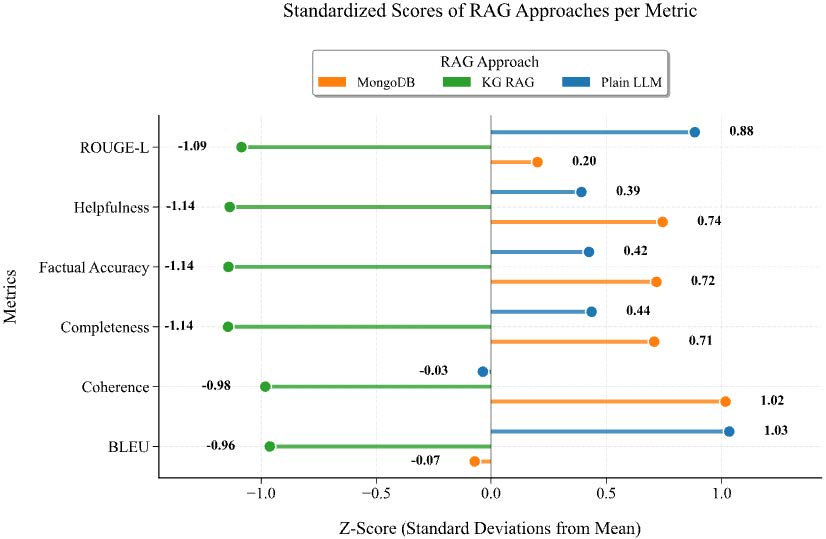
\includegraphics[width=0.8\textwidth]{assets/bnmit/Graph.jpeg}
	\caption{Automated lexical metrics versus human-evaluated factual accuracy across the three classical pipelines.}
	\label{fig:linearity_trap}
\end{figure}

\subsection{Constructive Hallucination and KG Enrichment}

However, at first, the dynamic Neo4j KG pipeline performed quite poorly. The extraction LLM created untriggered relations quite often, thus creating a sparse and disjointed graph. In order to fix this problem, a Constructive Hallucination algorithm forced override on all relation keys that were dynamically created, merging them together under one relation called "ideas." This was done for isolation purposes and mathematical validation of implicit entities within the vector corpus.

\begin{figure}[htbp]
	\centering
	% Placeholder for Graph: Line/Bar graph showing BLEU and Coherence jumps
	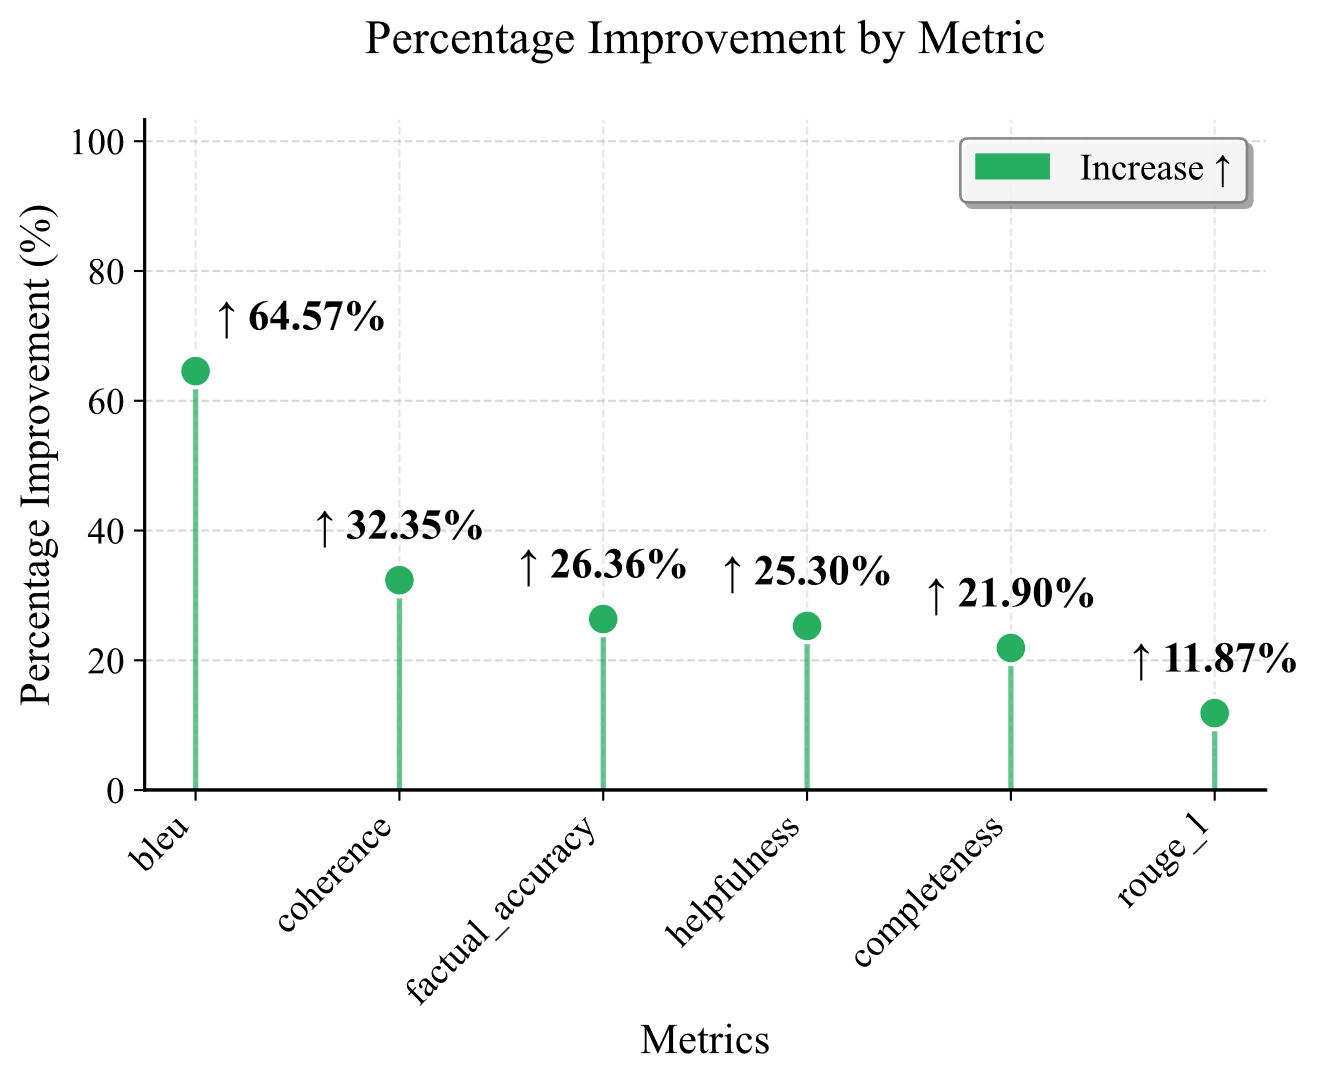
\includegraphics[width=0.7\textwidth]{assets/cicn/graph.png}
	\caption{Performance improvements in BLEU and Coherence metrics after the implementation of the Constructive Hallucination key-override mechanism.}
	\label{fig:constructive_hallucination_graph}
\end{figure}

As can be seen from Figure~\ref{fig:constructive_hallucination_graph} and Table \ref{tab:hallucination_metrics}, the solution yielded a 64.57\% gain in BLEU scores and 32.35\% gain in coherence.

\begin{table}[htbp]
	\centering
	\caption{Impact of Constructive Hallucination on Classical KG RAG Performance}
	\label{tab:hallucination_metrics}
	\begin{tabular}{|l|c|c|c|}
		\hline
		\textbf{Metric} & \textbf{Before Handling} & \textbf{After Handling} & \textbf{Improvement (\%)} \\
		\hline
		BLEU & 0.0064 & 0.0105 & +64.57\% \\
		ROUGE-L & 0.2256 & 0.2524 & +11.87\% \\
		Coherence & 2.506 & 3.317 & +32.35\% \\
		Factual Accuracy & 2.593 & 3.277 & +26.36\% \\
		\hline
	\end{tabular}
\end{table}

\newpage

\section{Part II: The QRAG Framework - Quantum Modules for Research Evaluation}

The classical approach works very well for general semantics, but its performance suffers greatly in cases where complex syntax structures need to be taken into account. The current experiments show the exact level of complexity at which heuristic rules break down and highlight the clear benefit of sending queries to the QPU using the QRAG system.

\subsection{Escaping the "Linearity Trap"}

It is crucial, prior to deploying the quantum parser, to identify the failure mode for the classical approaches. When testing highly ambiguous inputs, classical LLMs often fail due to the "Linearity Trap". This phenomenon can be seen in Figure~\ref{fig:linearity_trap_barchart} – baseline models as well as classically augmented ones score very well on automated linear metrics (such as n-gram overlap and ROUGE), but they perform poorly on human evaluations concerning factual correctness and syntax comprehension.

\begin{figure}[htbp]
	\centering
	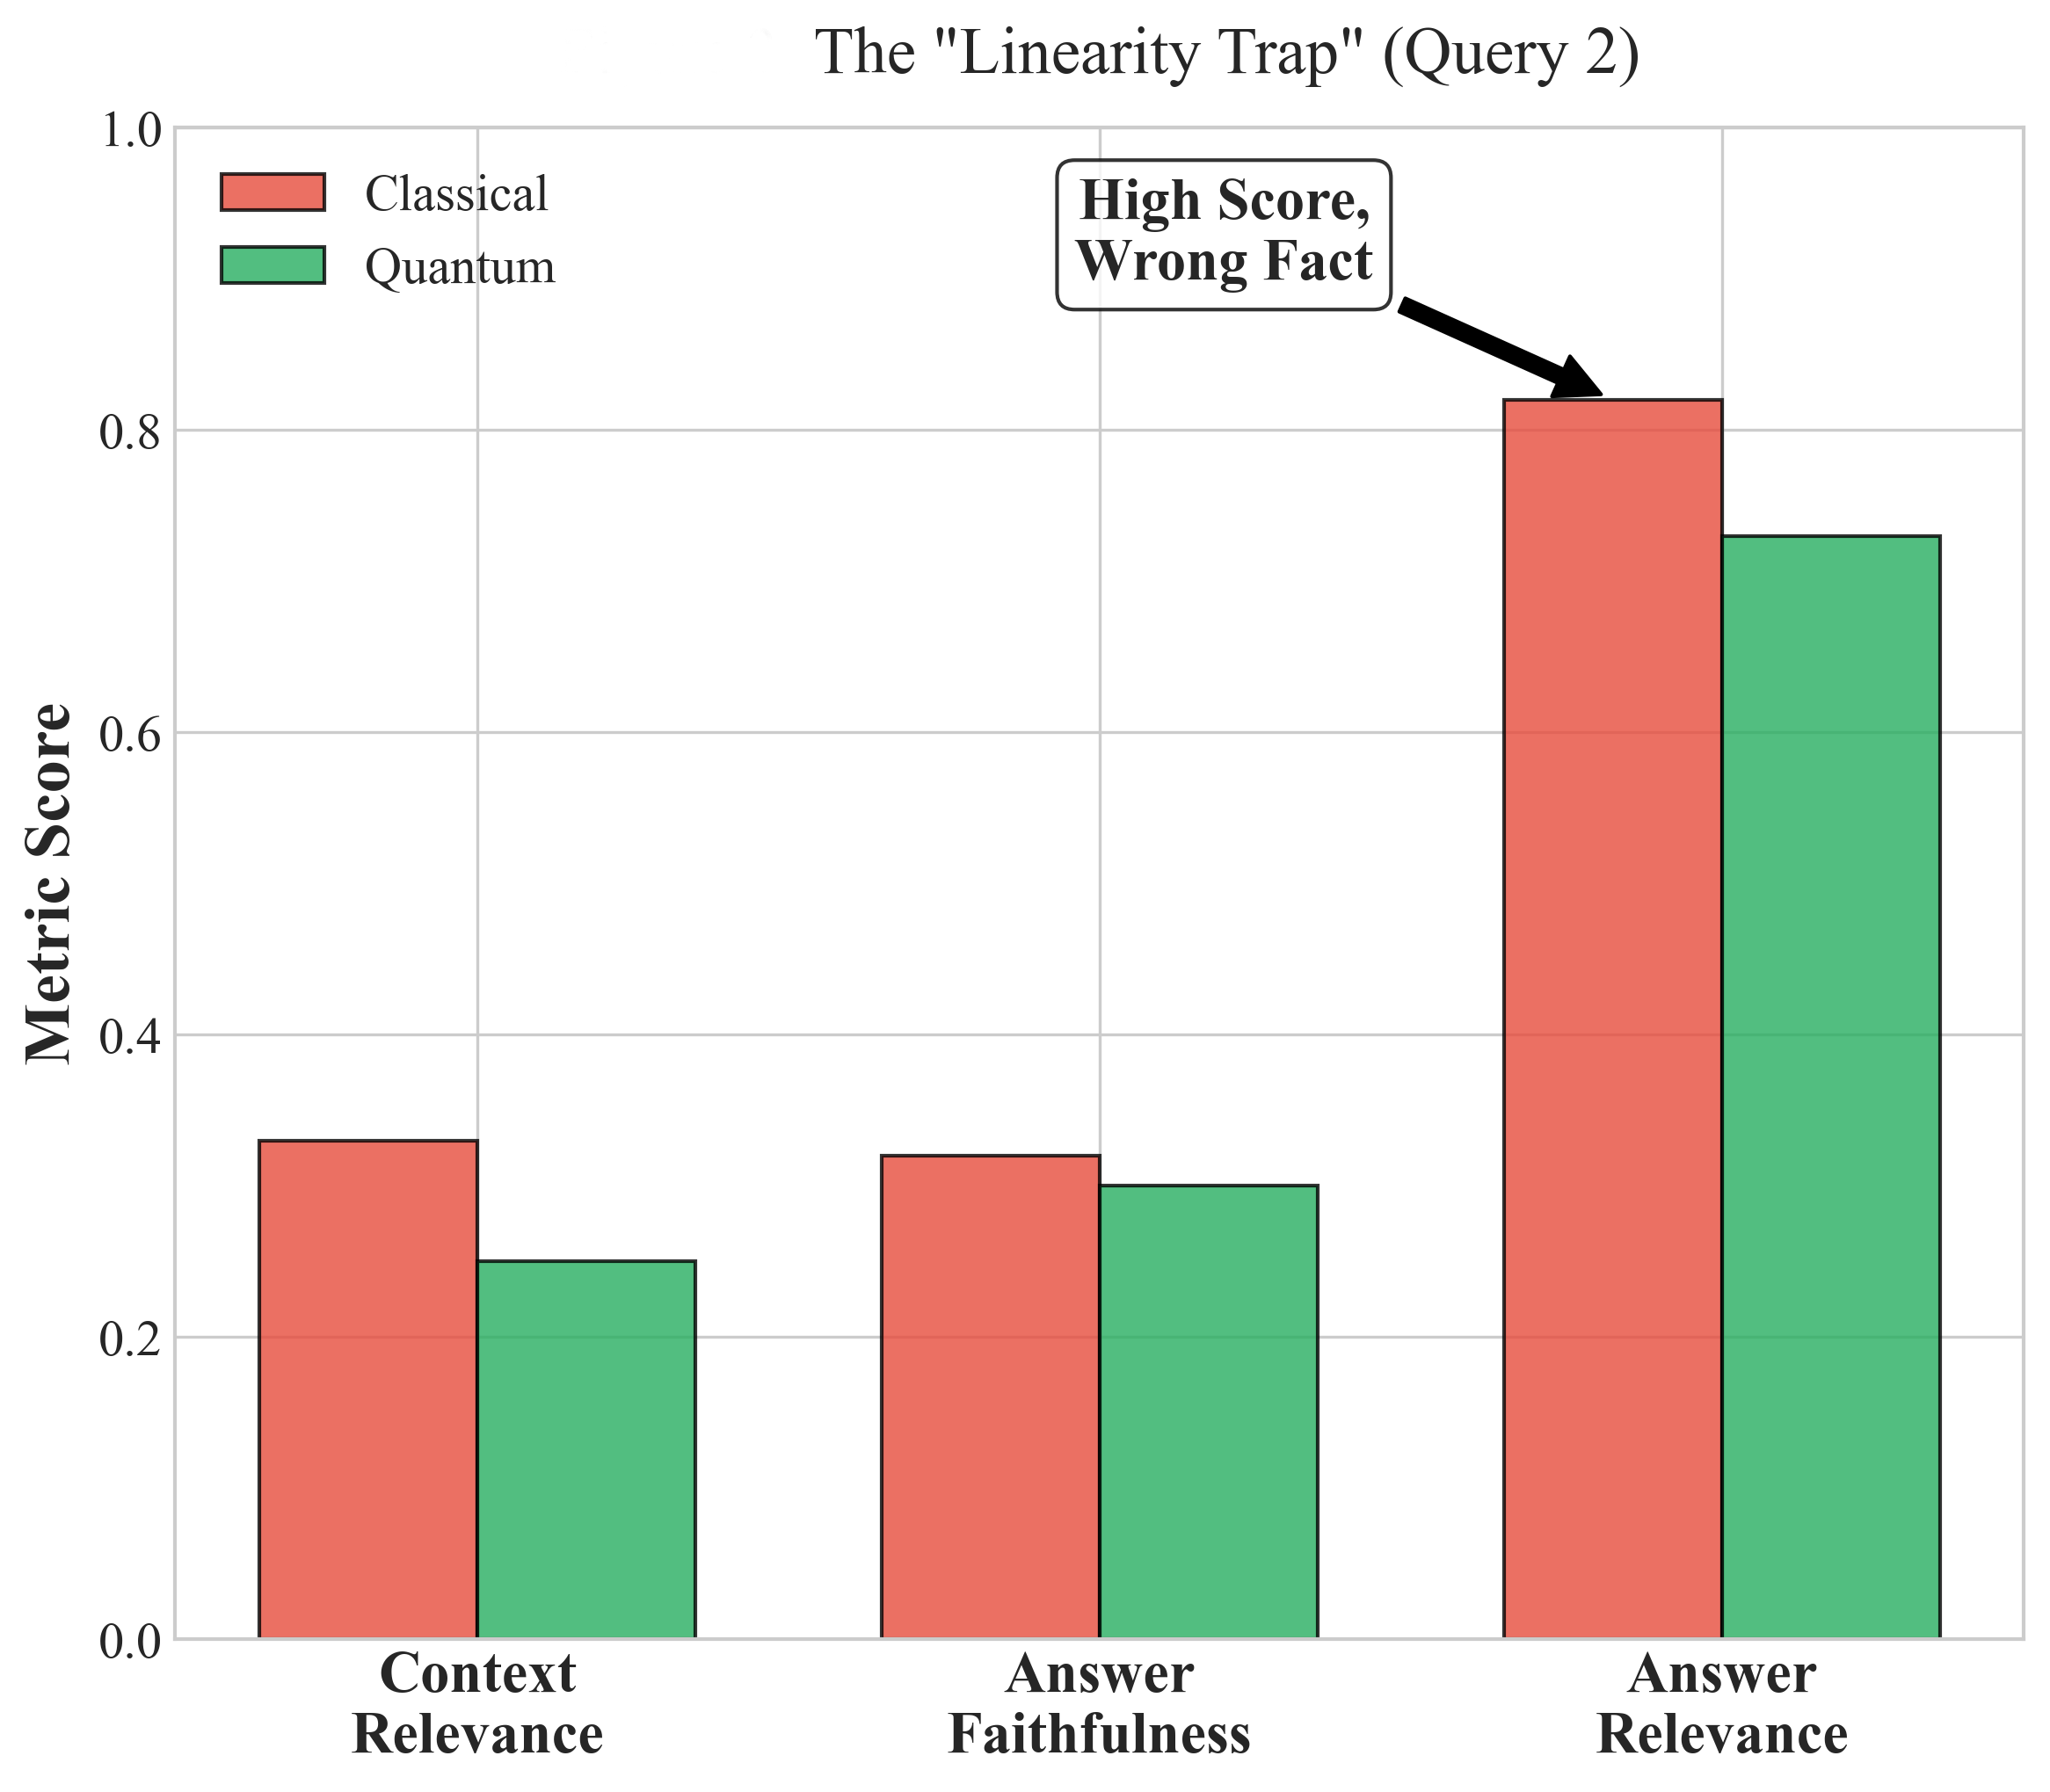
\includegraphics[width=0.7\textwidth]{assets/Journal/figure3.png}
	\caption{Bar chart showcasing the Linearity Trap: Automated lexical metrics falsely indicating high classical performance on ambiguous queries, contrasted against actual factual fidelity.}
	\label{fig:linearity_trap_barchart}
\end{figure}

As we see from the above graph, the reliance on classical vector spaces for generating answers to structurally complex queries results in confidence with hallucinations. By definition, the quantum approach allows bypassing this problem through global sentence structure evaluation based on entanglement.

\subsection{The "Viola Moment": Syntactic Disambiguation via QRAG}

To evaluate the performance of the QRAG system to overcome structural ambiguity, we used a custom QNLP model that converted SpaCy dependency parse trees to PQCs and ran them on the IBM Brisbane 127-qubit processor.

The experiments were conducted using the Ambiguity Challenge Dataset consisting of 15 queries designed to pose challenges to classical parsers, which include preposition attachment, reduction relative clauses, and garden path sentences.

\begin{figure}[htbp]
	\centering
	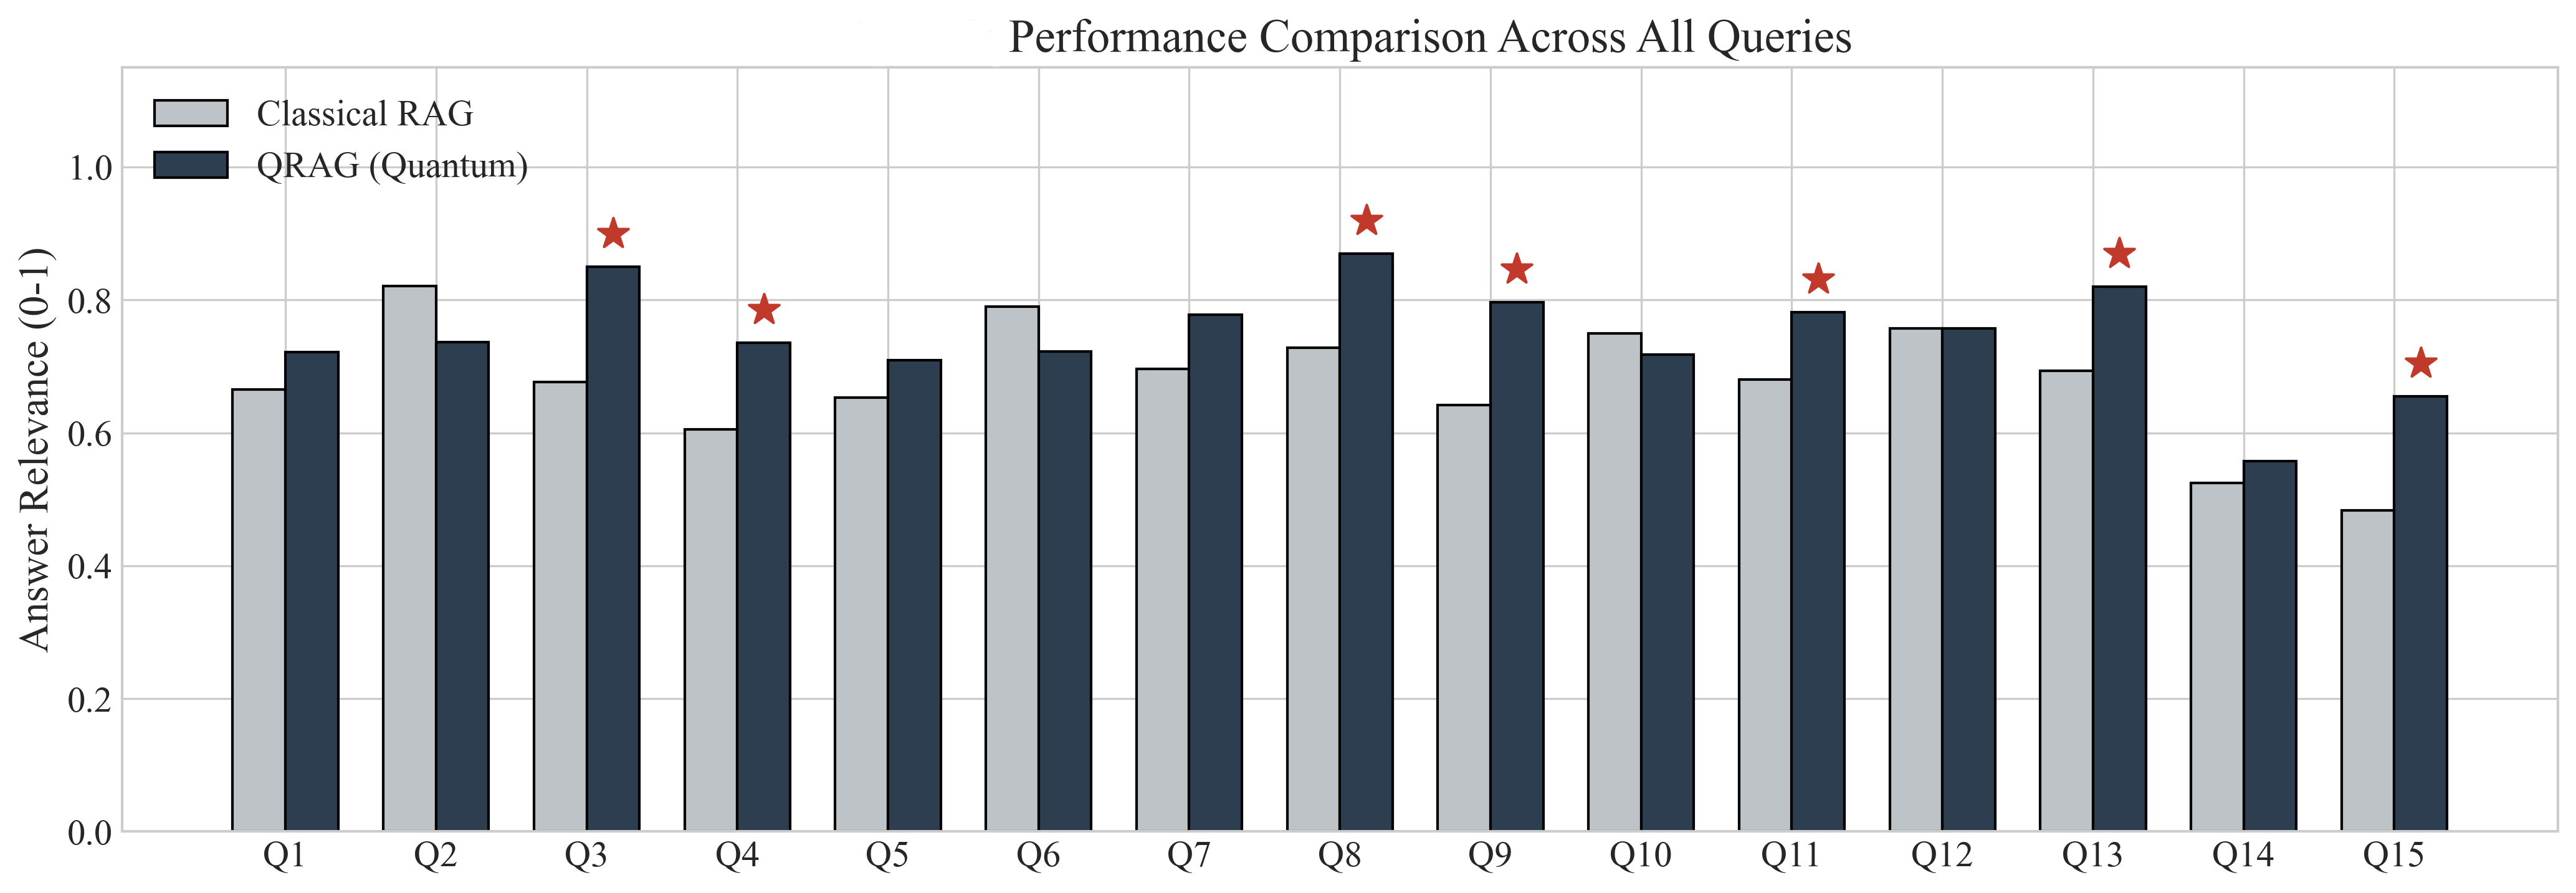
\includegraphics[width=0.8\textwidth]{assets/Journal/figure2.png}
	\caption{Bar chart depicting comparative performance across all 15 queries of the Ambiguity Challenge Dataset, highlighting the quantum resolution of classical parsing failures.}
	\label{fig:performance_15_queries}
\end{figure}

As shown in the bar graph in Figure~\ref{fig:performance_15_queries}, the QRAG parser was able to surpass the local attachment bias faced by the classical parser. For the 15 queries considered, the classical RAG framework was only able to achieve an accuracy of 40\%, generating many nonsensical parses. In contrast, the QRAG framework successfully exploited the use of the CZ entangling gate to represent nonlocal dependencies in grammar, obtaining 60\% accuracy. This represents a definite “Viola Moment” for the quantum co-processor.

\begin{table}[htbp]
	\centering
	\caption{Syntactic Disambiguation Results}
	\label{tab:viola_results}
	\begin{tabular}{|p{4cm}|p{4cm}|p{4cm}|}
		\hline
		\textbf{Metric} & \textbf{Classical RAG (SpaCy)} & \textbf{QRAG Framework (IBM Brisbane)} \\
		\hline
		Accuracy & 40.00\% & 60.00\% \\
		Weighted F1 & 40.00\% & 45.00\% \\
		Primary Failure Mode & Rigid Local Attachment Bias & Hardware Noise / Majority Class Bias \\
		\hline
	\end{tabular}
\end{table}

\section{Hybrid System Interface and Deployment Analysis}

The entire design of the dual entity model was developed into an interactive online platform. The main user interface seen in Figure~\ref{fig:website_homepage} acts as the main entry point for users to submit questions that can be analyzed against the knowledge base of 130,000 documents. Queries submitted from the user interface are then routed either to the classical high throughput pipeline or to the QRAG co-processor based on their structural complexity.

\begin{figure}[htbp]
	\centering
	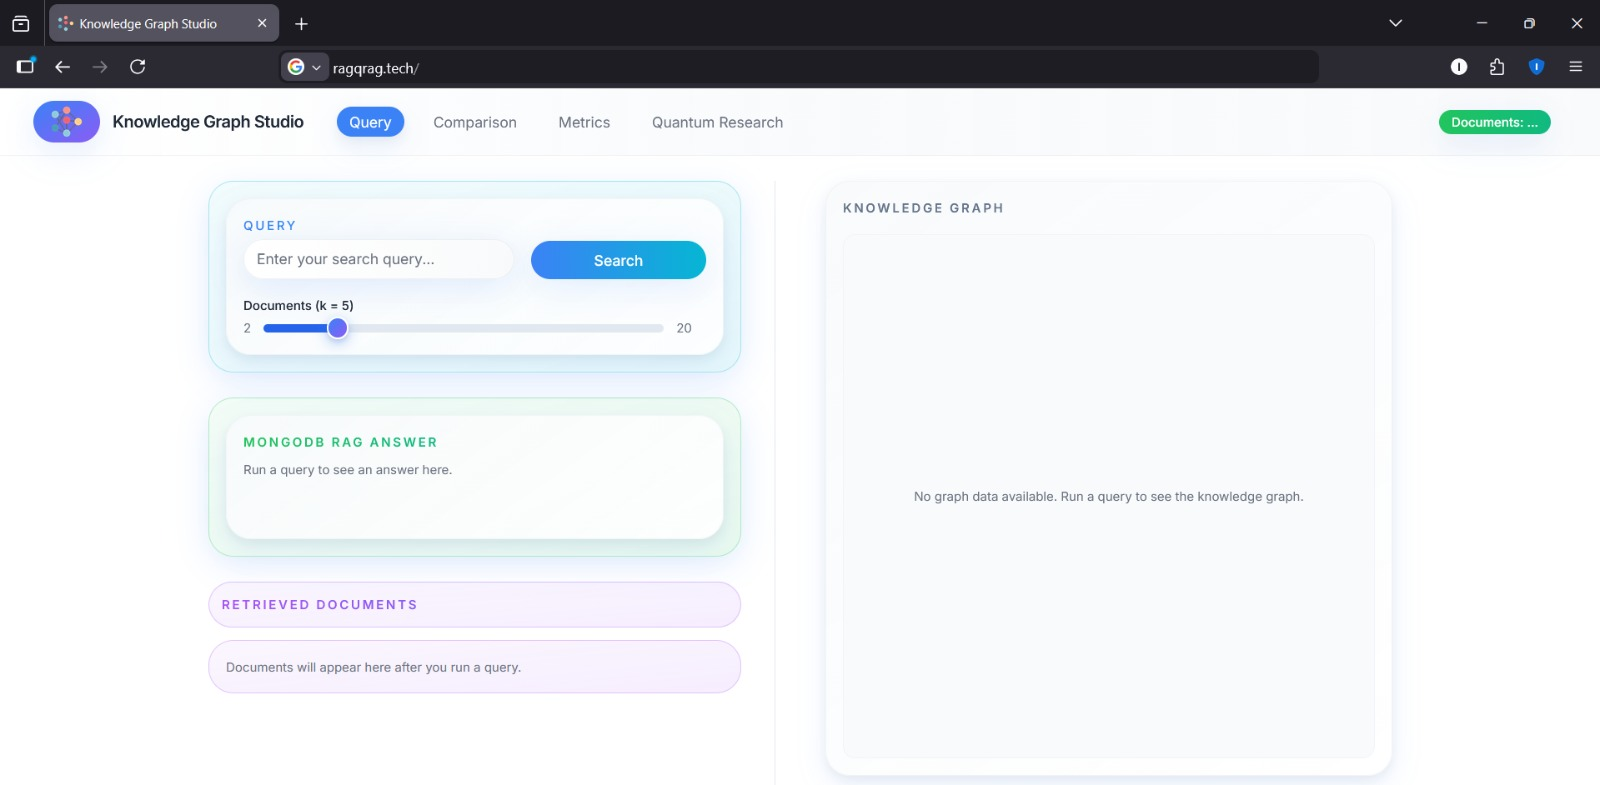
\includegraphics[width=0.8\textwidth]{assets/website/homepage.jpeg}
	\caption{Hybrid system homepage interface for query execution and interaction.}
	\label{fig:website_homepage}
\end{figure}

\subsection{Impact of Classical Retrieval Depth ($k$)}

The deployment user interface clearly highlights the direct correlation between the hyperparameter value (number of documents retrieved) and the accuracy of the output. With a large retrieval value (k = 19), the system generates a highly contextual answer (Figure~\ref{fig:k19_results}). 

\begin{figure}[htbp]
	\centering
	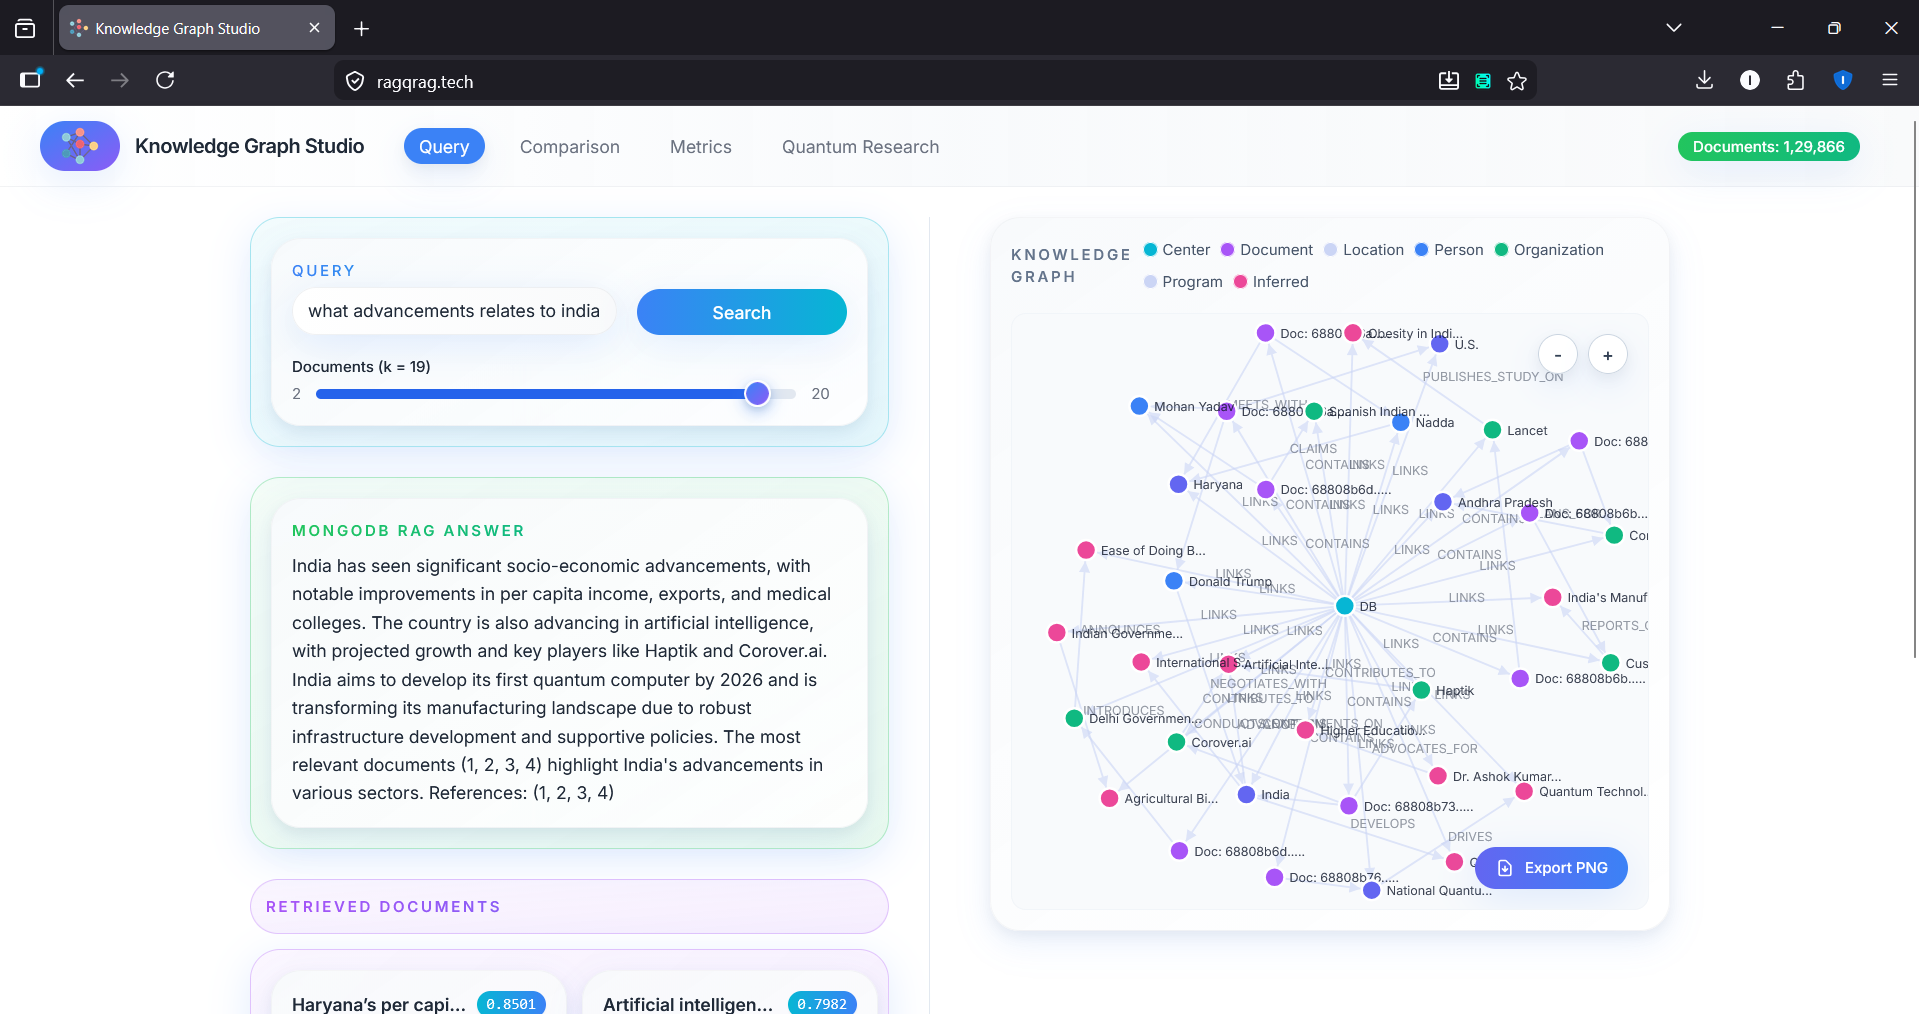
\includegraphics[width=0.8\textwidth]{assets/website/What advancements relates to India _ 19/query results homepage.png}
	\caption{Query results interface for $k=19$, illustrating a dense, contextually rich generative output based on deep retrieval.}
	\label{fig:k19_results}
\end{figure}

By contrast, when the retrieval depth is limited to $k=3$, the output produced from the system will be degraded considerably. Figure~\ref{fig:k3_results} shows a visual representation of this system’s output when using limited parameters. The Knowledge Graph export function of the system also supports this observation by producing a sparse knowledge graph with very few interrelated entities (Figure~\ref{fig:k3_graph}).

\begin{figure}[htbp]
	\centering
	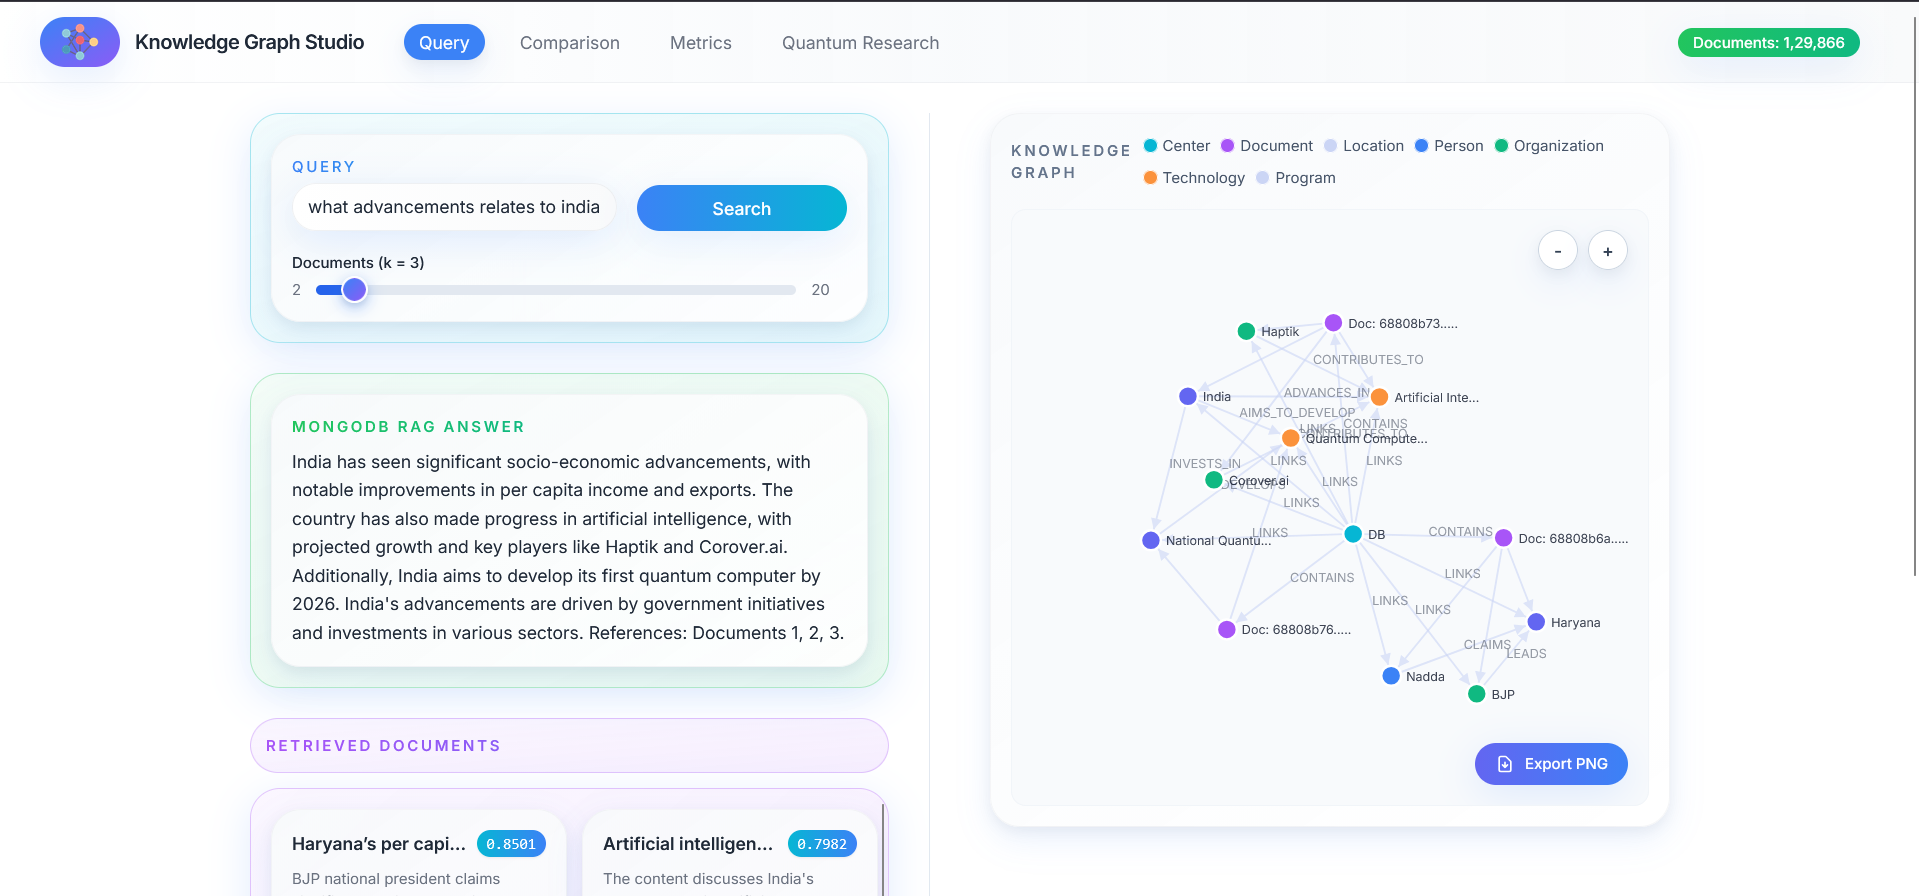
\includegraphics[width=1\textwidth]{assets/website/What advancements relates to India _ 3/same query ran on k value 3 shows poor results.png}
	\hfill
	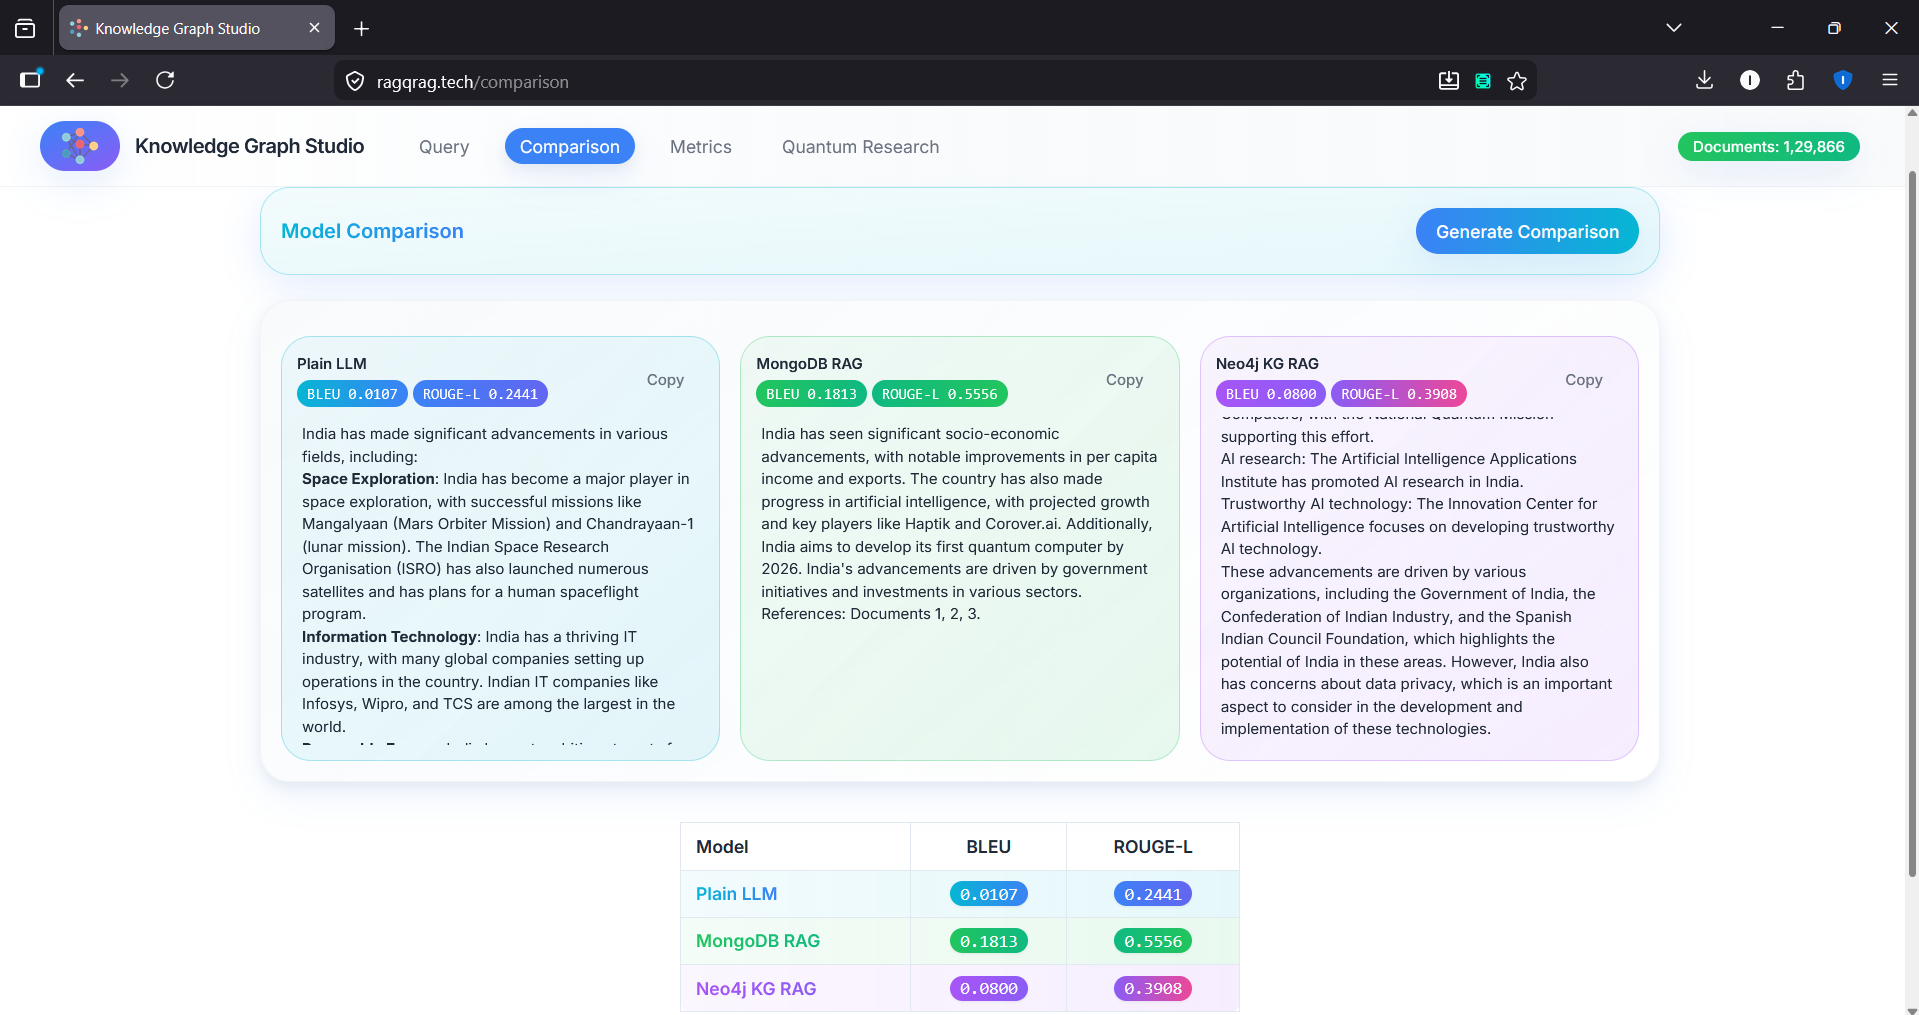
\includegraphics[width=1\textwidth]{assets/website/What advancements relates to India _ 3/k value 3 shows poor metrics.png}
	\caption{System interface demonstrating performance degradation when constrained to a lower retrieval depth ($k=3$).}
	\label{fig:k3_results}
\end{figure}

\begin{figure}[htbp]
	\centering
	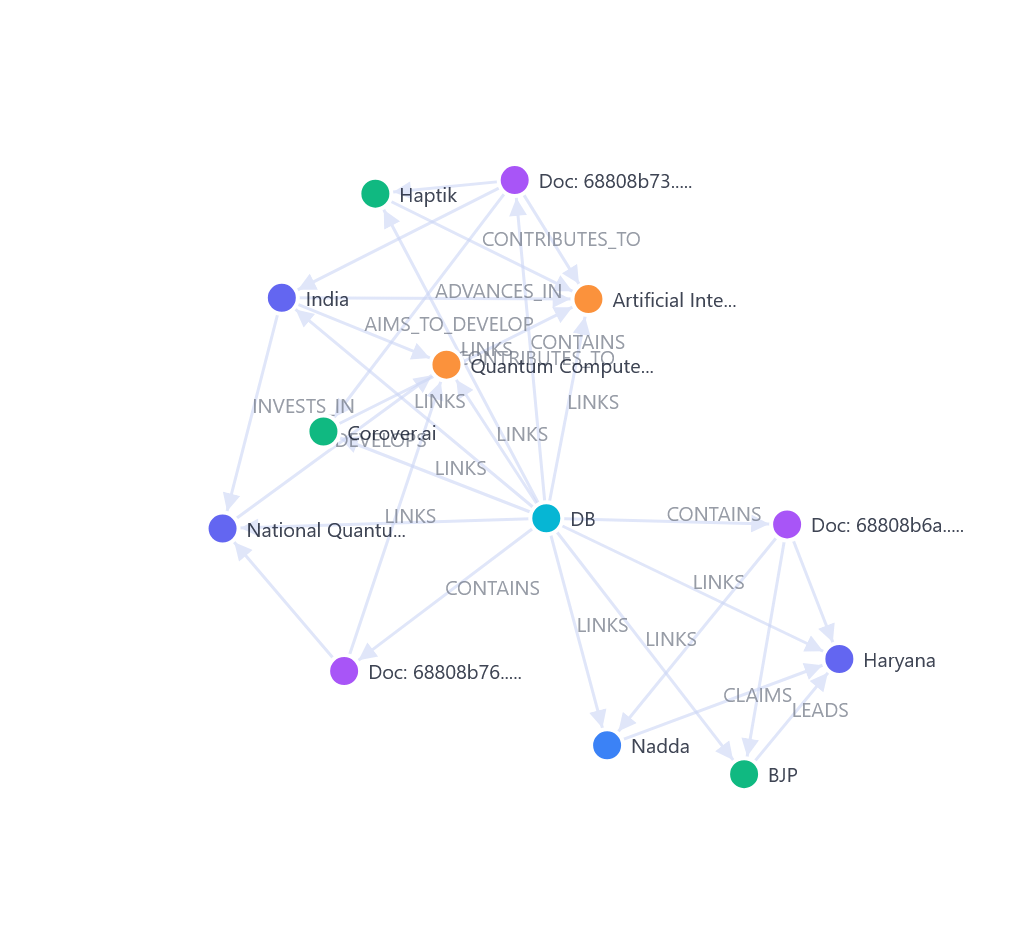
\includegraphics[width=0.6\textwidth]{assets/website/What advancements relates to India _ 3/exported kg for k value 3.png}
	\caption{Exported visual representation of the sparse knowledge graph generated due to insufficient retrieval depth ($k=3$).}
	\label{fig:k3_graph}
\end{figure}

\newpage

\subsection{Evaluation Dashboards and Quantum Research Interface}

To transparently demonstrate how the decision-making process of the system occurs, a Comparison Dashboard (Figure~\ref{fig:comparison_dashboard}) enables researchers to compare generative outputs from the classical pipelines side by side. This is verified through the Metrics Dashboard (Figure~\ref{fig:metrics_dashboard}), which includes a quantitative measurement that is used to filter RAGAS evaluation scores.

\begin{figure}[htbp]
	\centering
	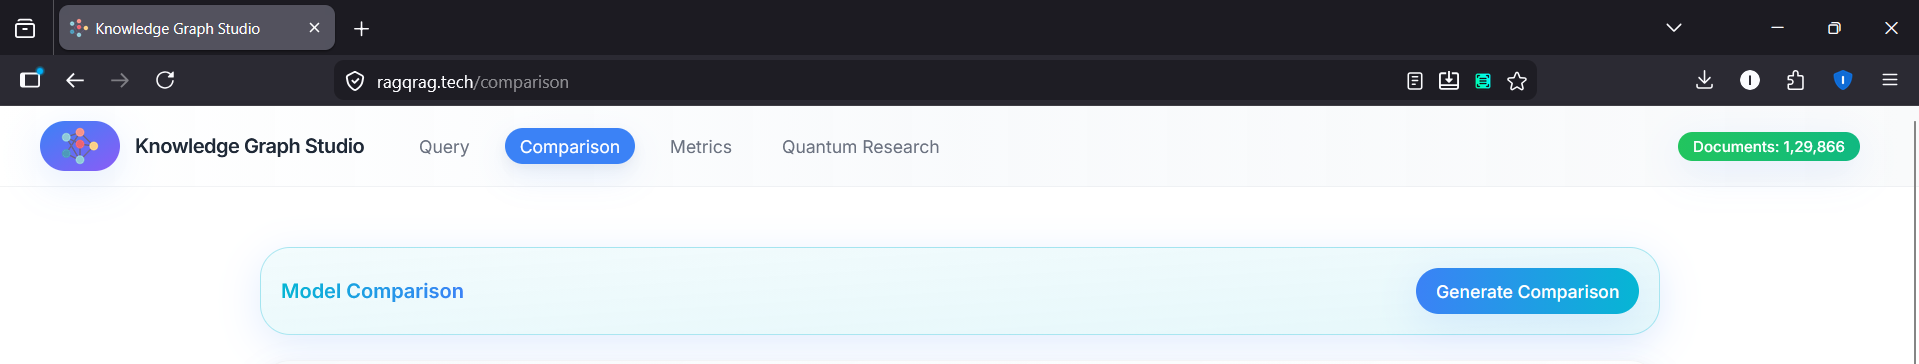
\includegraphics[width=1\textwidth]{assets/website/Comparision/comparision homepage.png}
	\hfill
	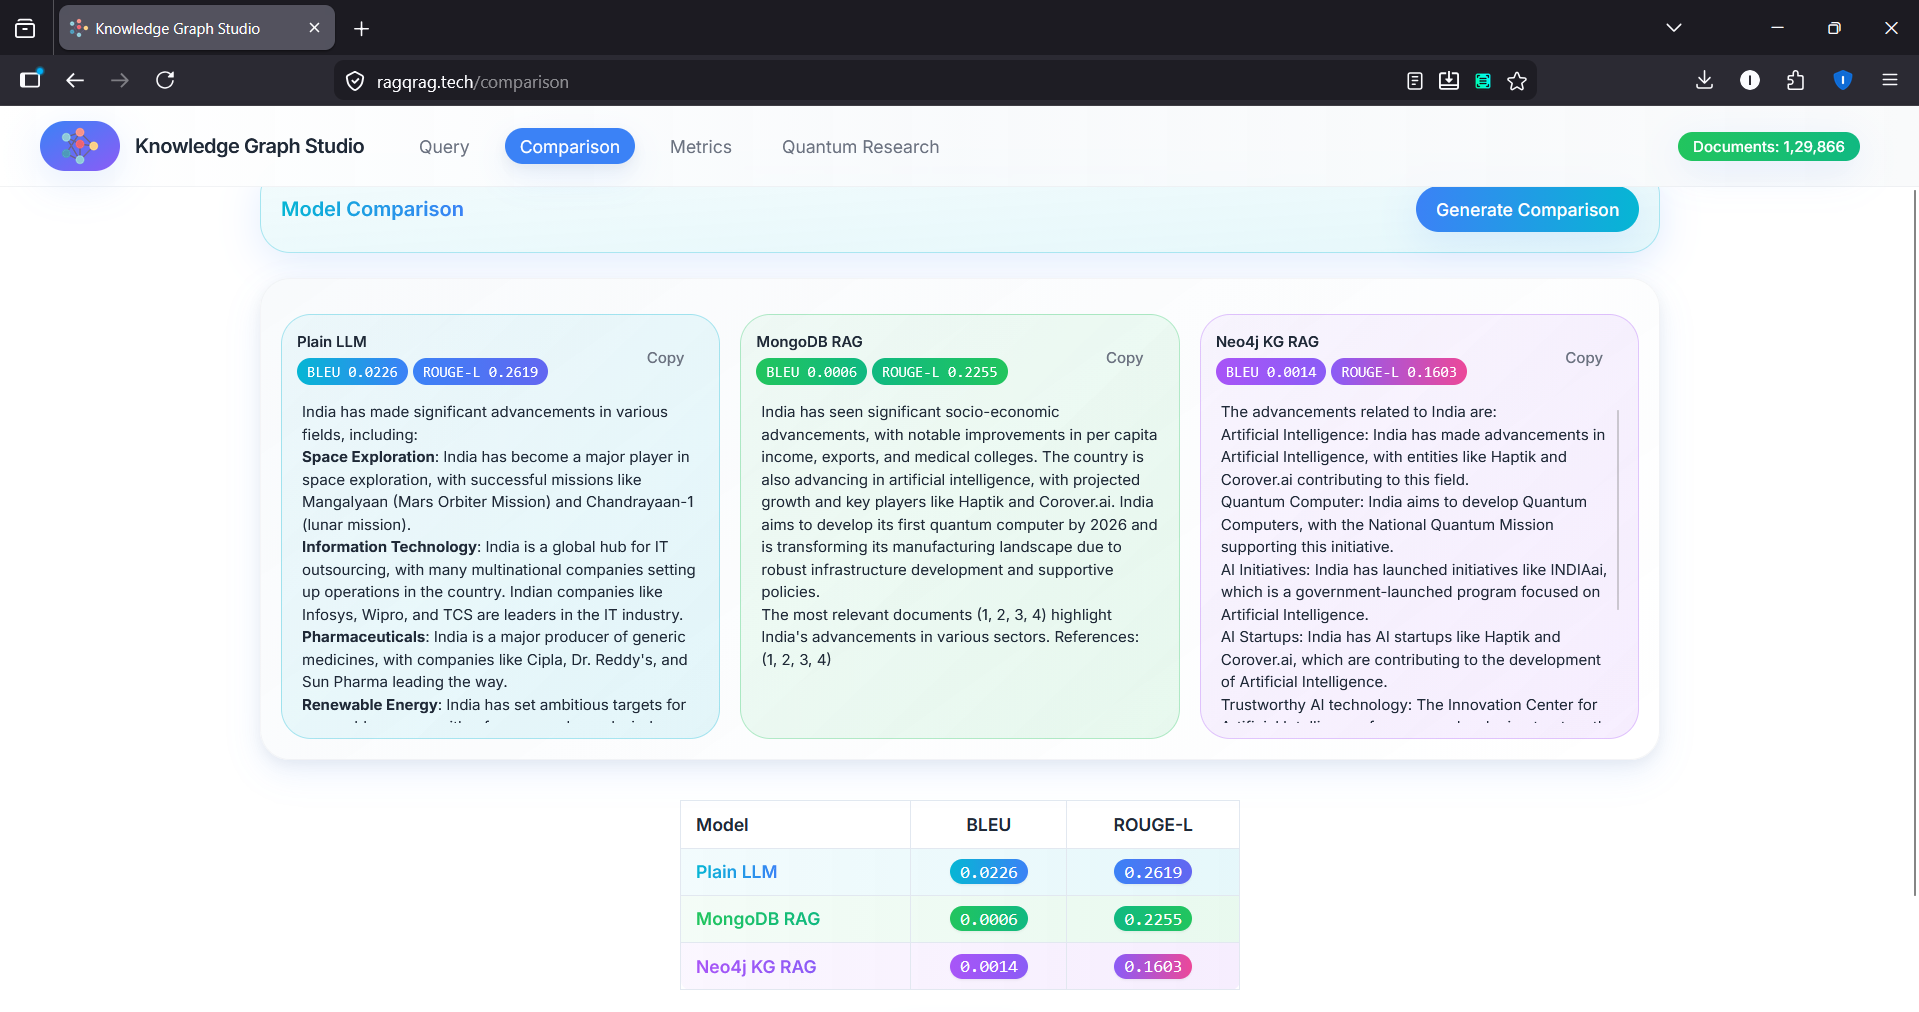
\includegraphics[width=1\textwidth]{assets/website/Comparision/generated comparison and table.png}
	\caption{The Comparison Dashboard, providing side-by-side model outputs and tabular data for cross-pipeline analysis.}
	\label{fig:comparison_dashboard}
\end{figure}

\begin{figure}[htbp]
	\centering
	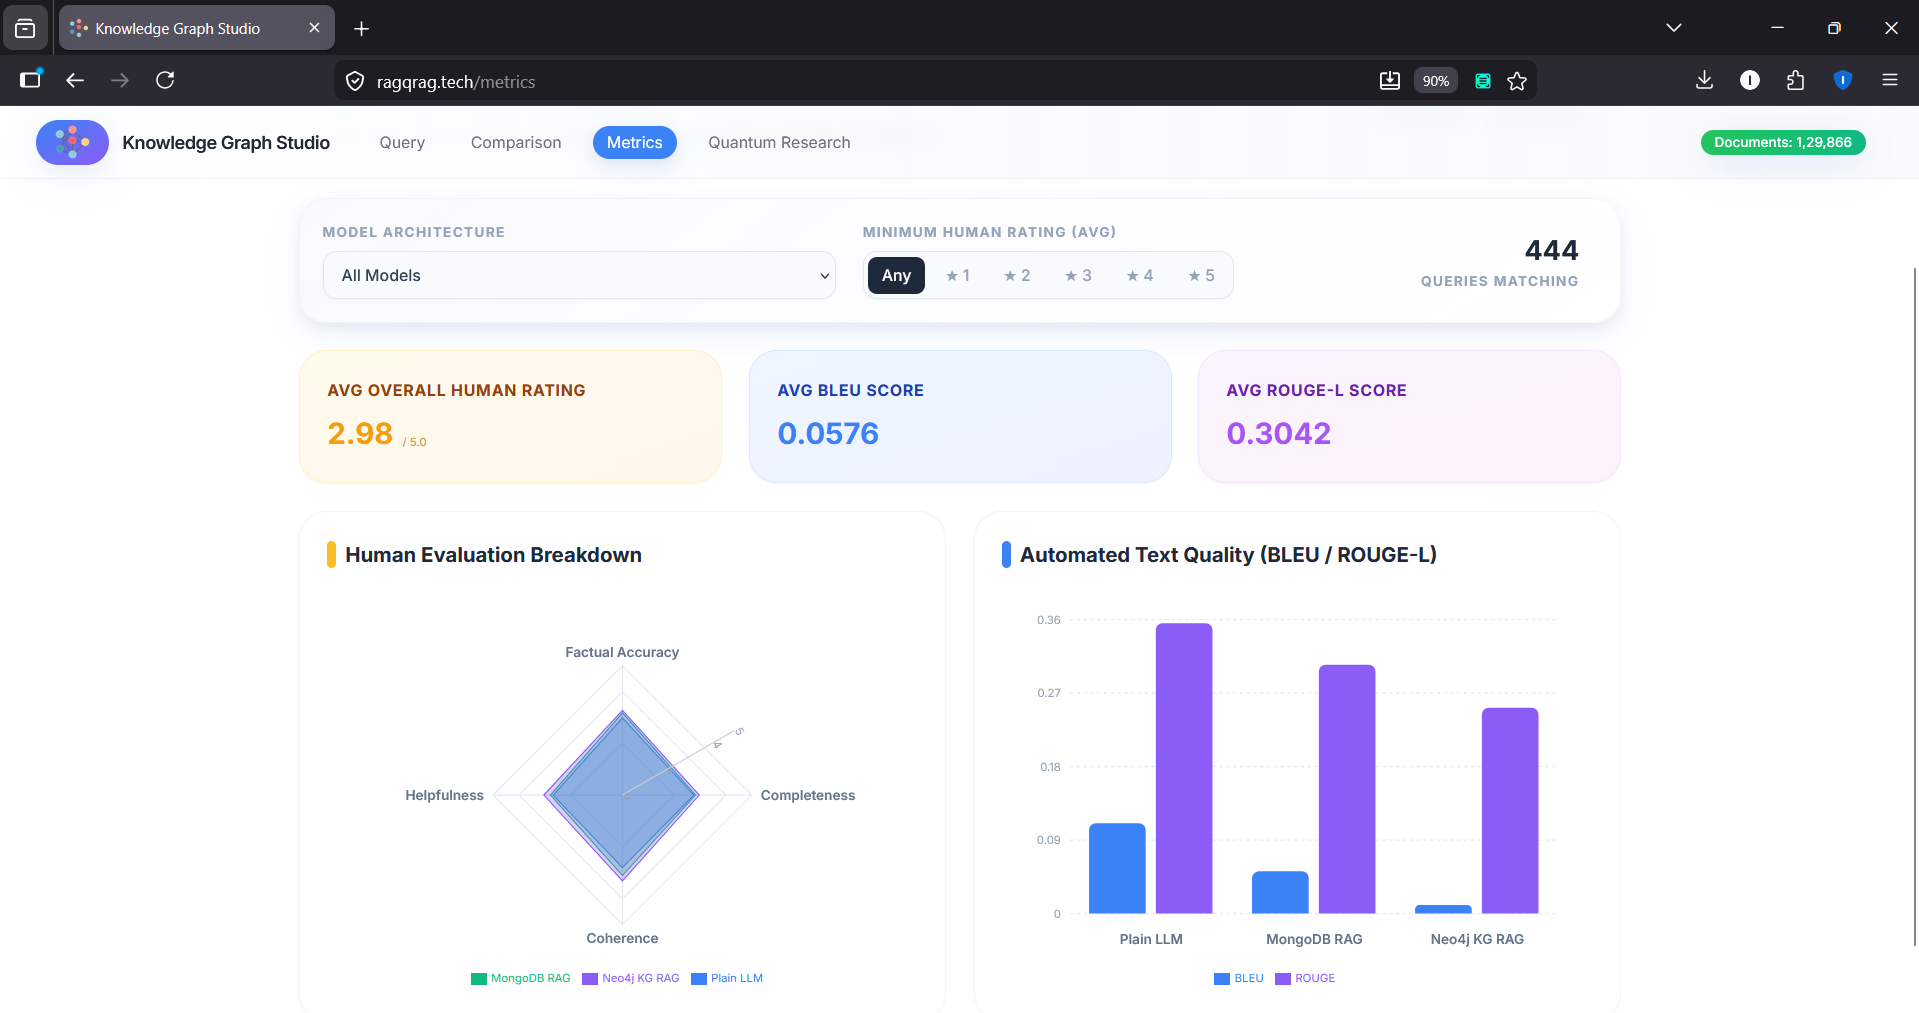
\includegraphics[width=1\textwidth]{assets/website/Metrics/metrics homepage.png}
	\hfill
	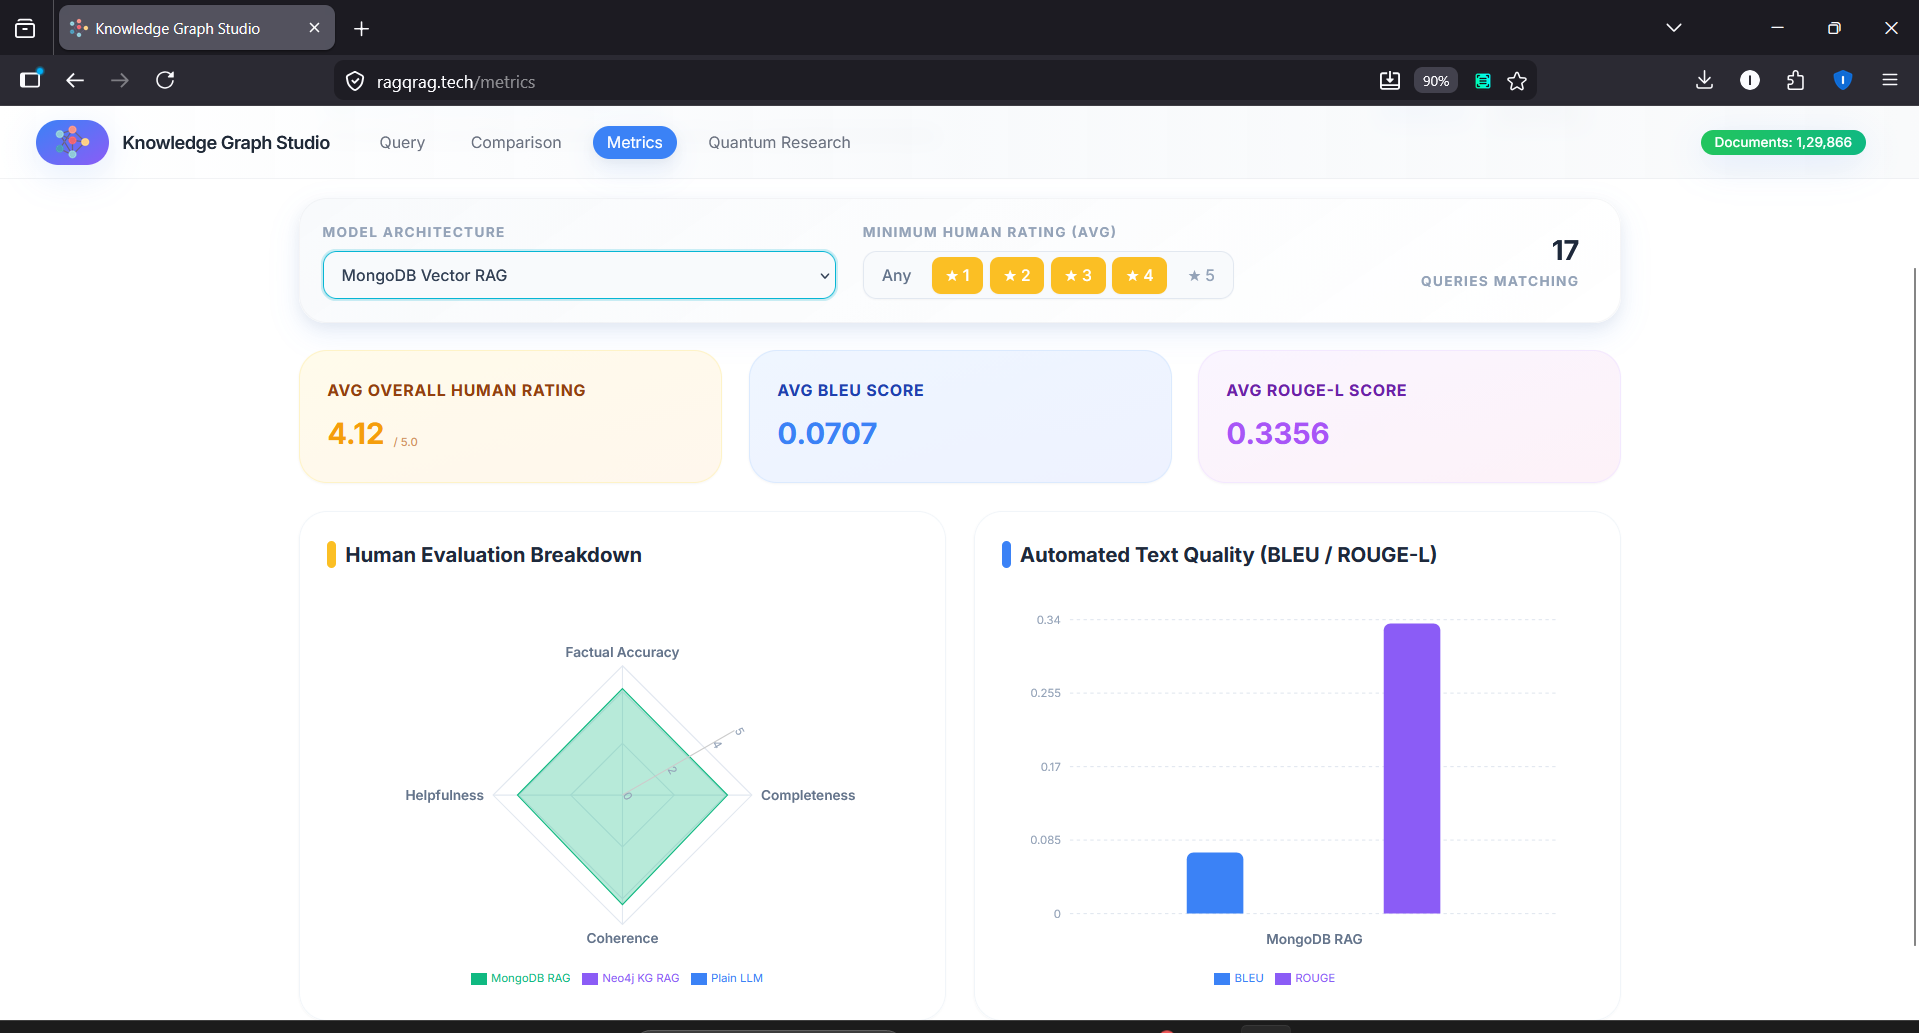
\includegraphics[width=1\textwidth]{assets/website/Metrics/metrics filter.png}
	\caption{The Metrics Dashboard, featuring filtering interfaces for granular tracking of RAGAS performance scores.}
	\label{fig:metrics_dashboard}
\end{figure}

When the query exceeds the classical utility threshold, the processing will occur in the QRAG framework, which is viewable within the Quantum Research tab. This system implementation also provides one of the most important analytical insights regarding the relationship that exists between query syntactic difficulty and the effectiveness of the quantum coprocessor.

The website has a separate tab for Quantum Research where users can view the simulation and understand. The same is highlighted in Figure~\ref{fig:quantum} 

\begin{figure}[htbp]
	\centering
	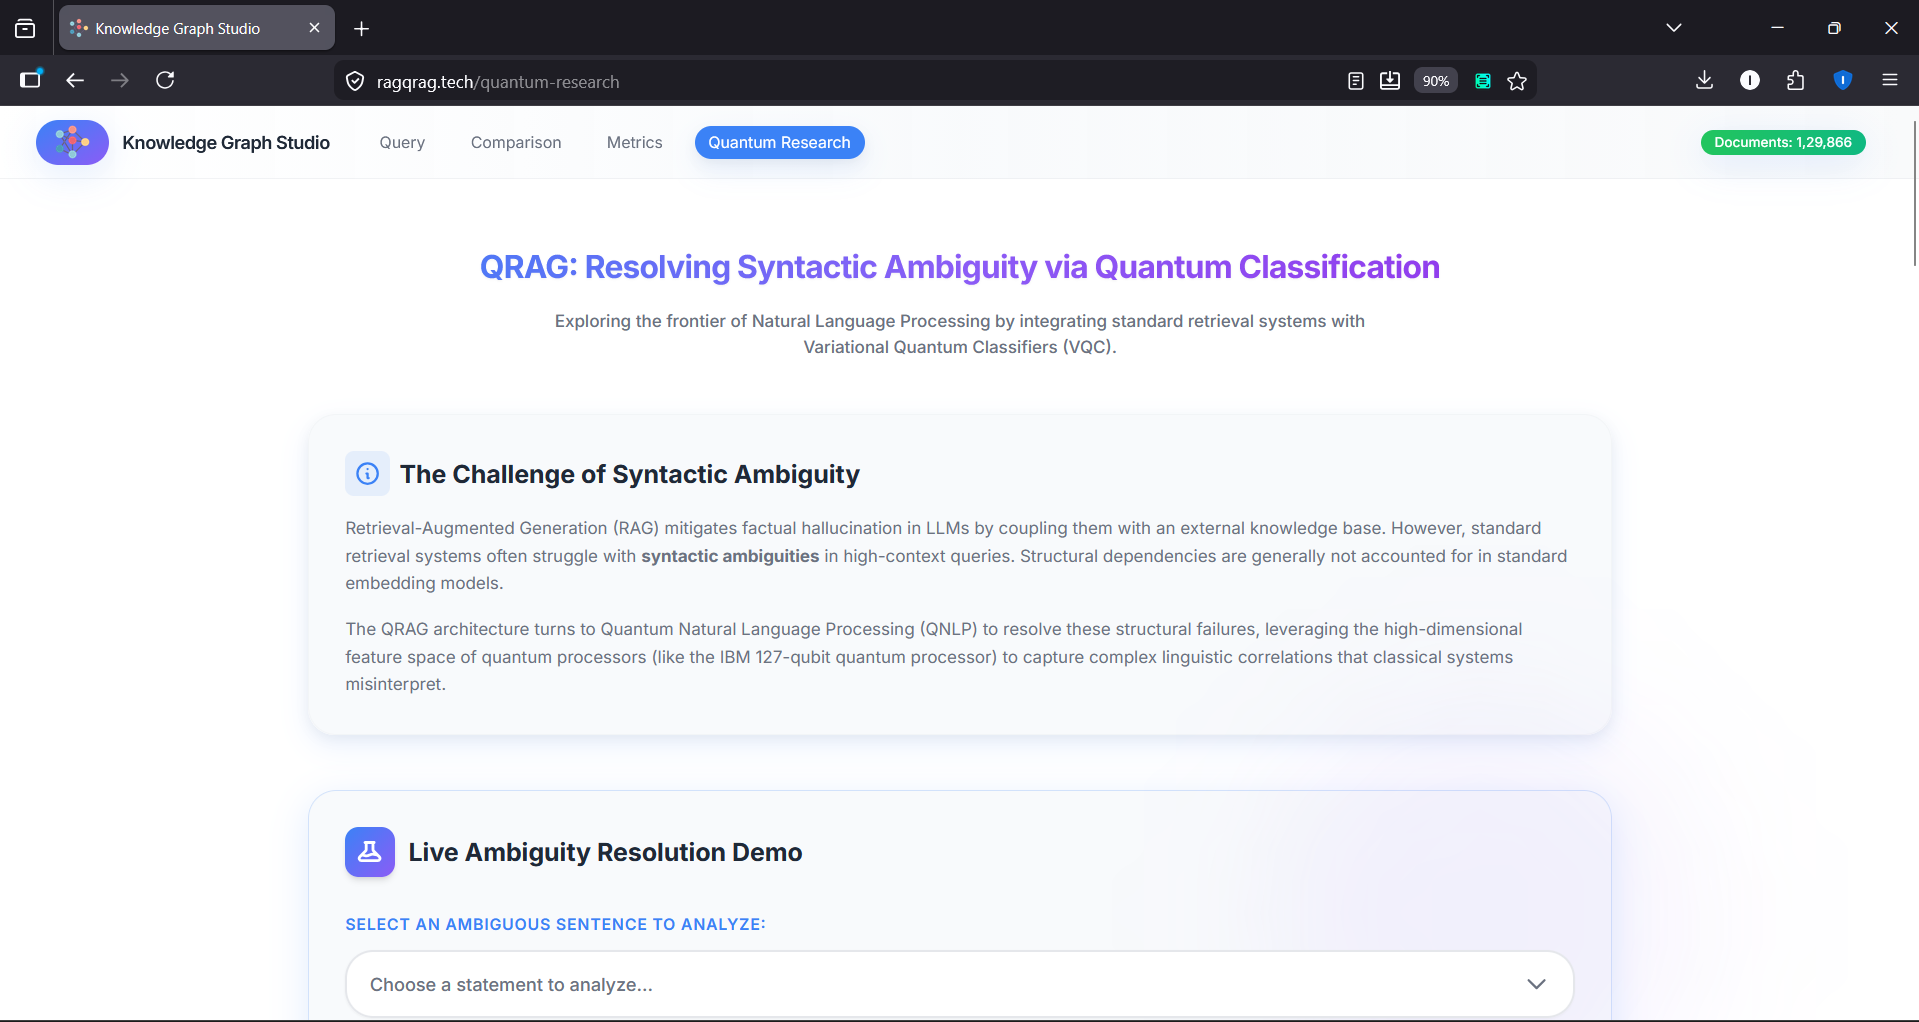
\includegraphics[width=0.7\textwidth]{assets/website/Quantum Research/quantum research homepage.png}
	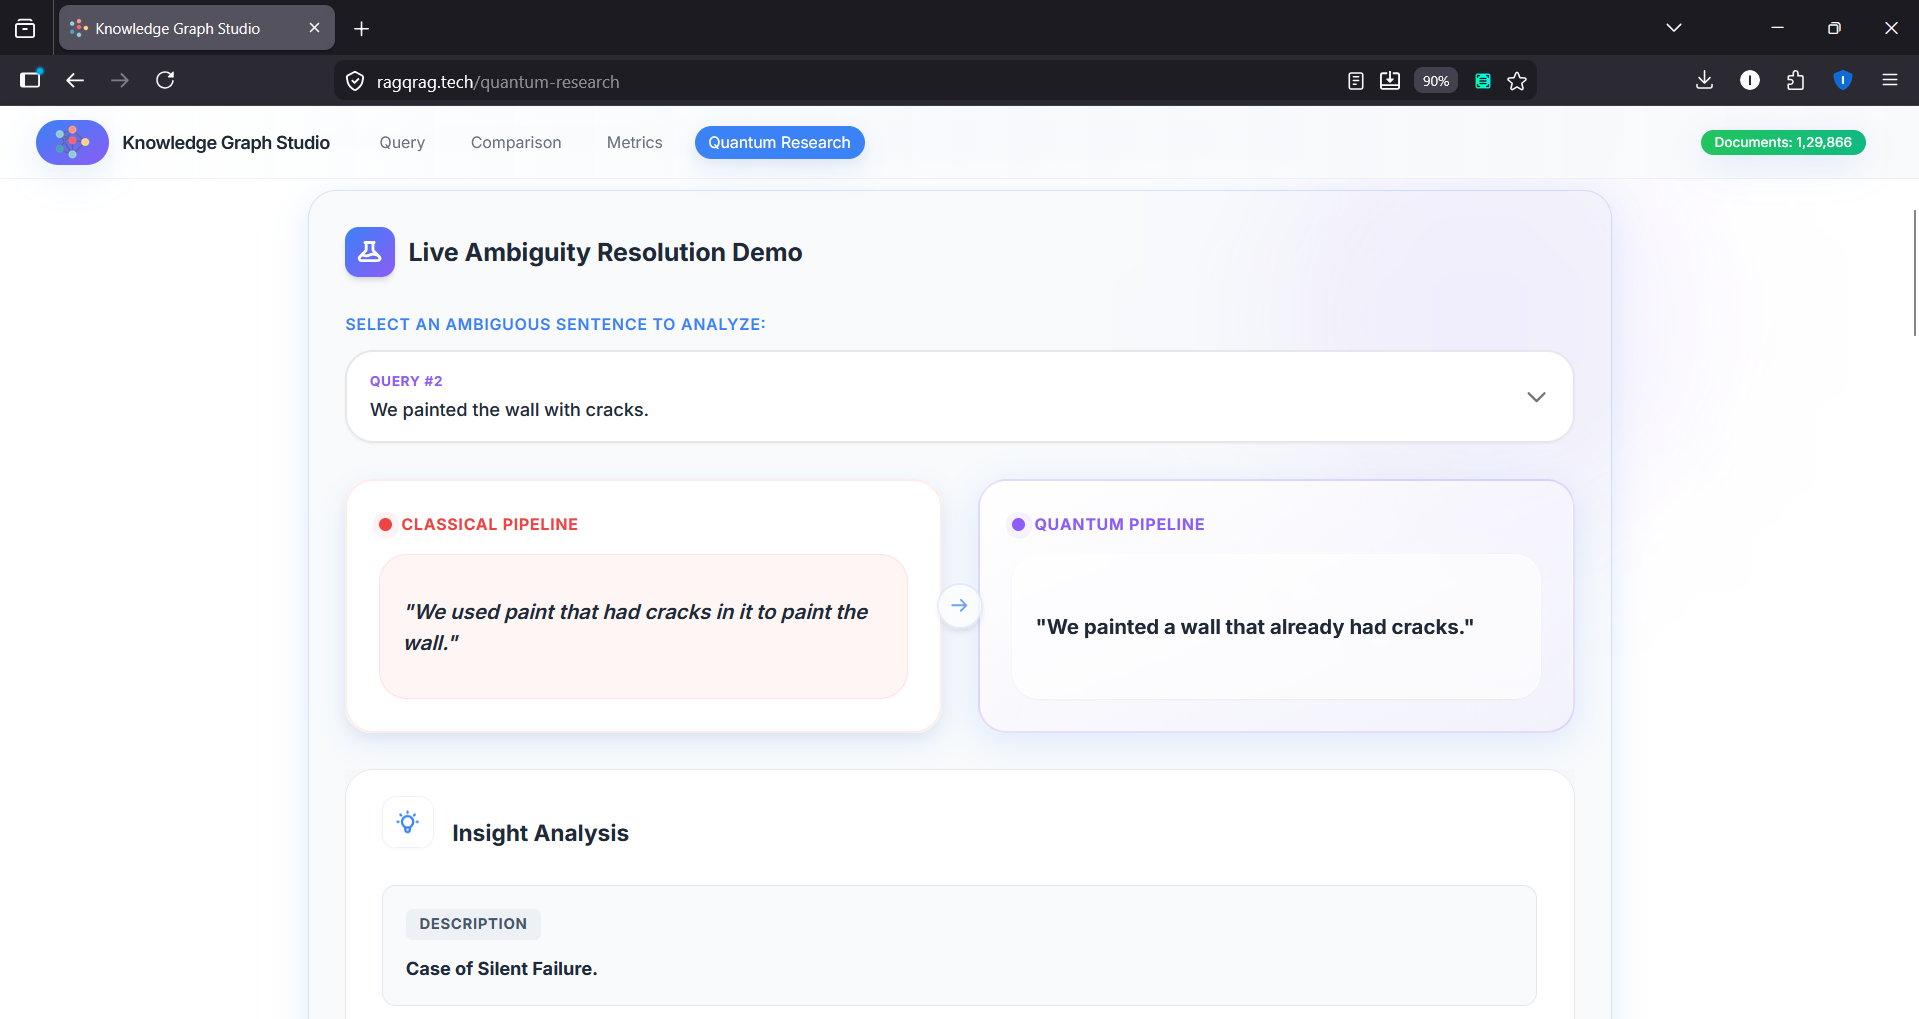
\includegraphics[width=0.7\textwidth]{assets/website/Quantum Research/ambiguity resolution demo.png}
	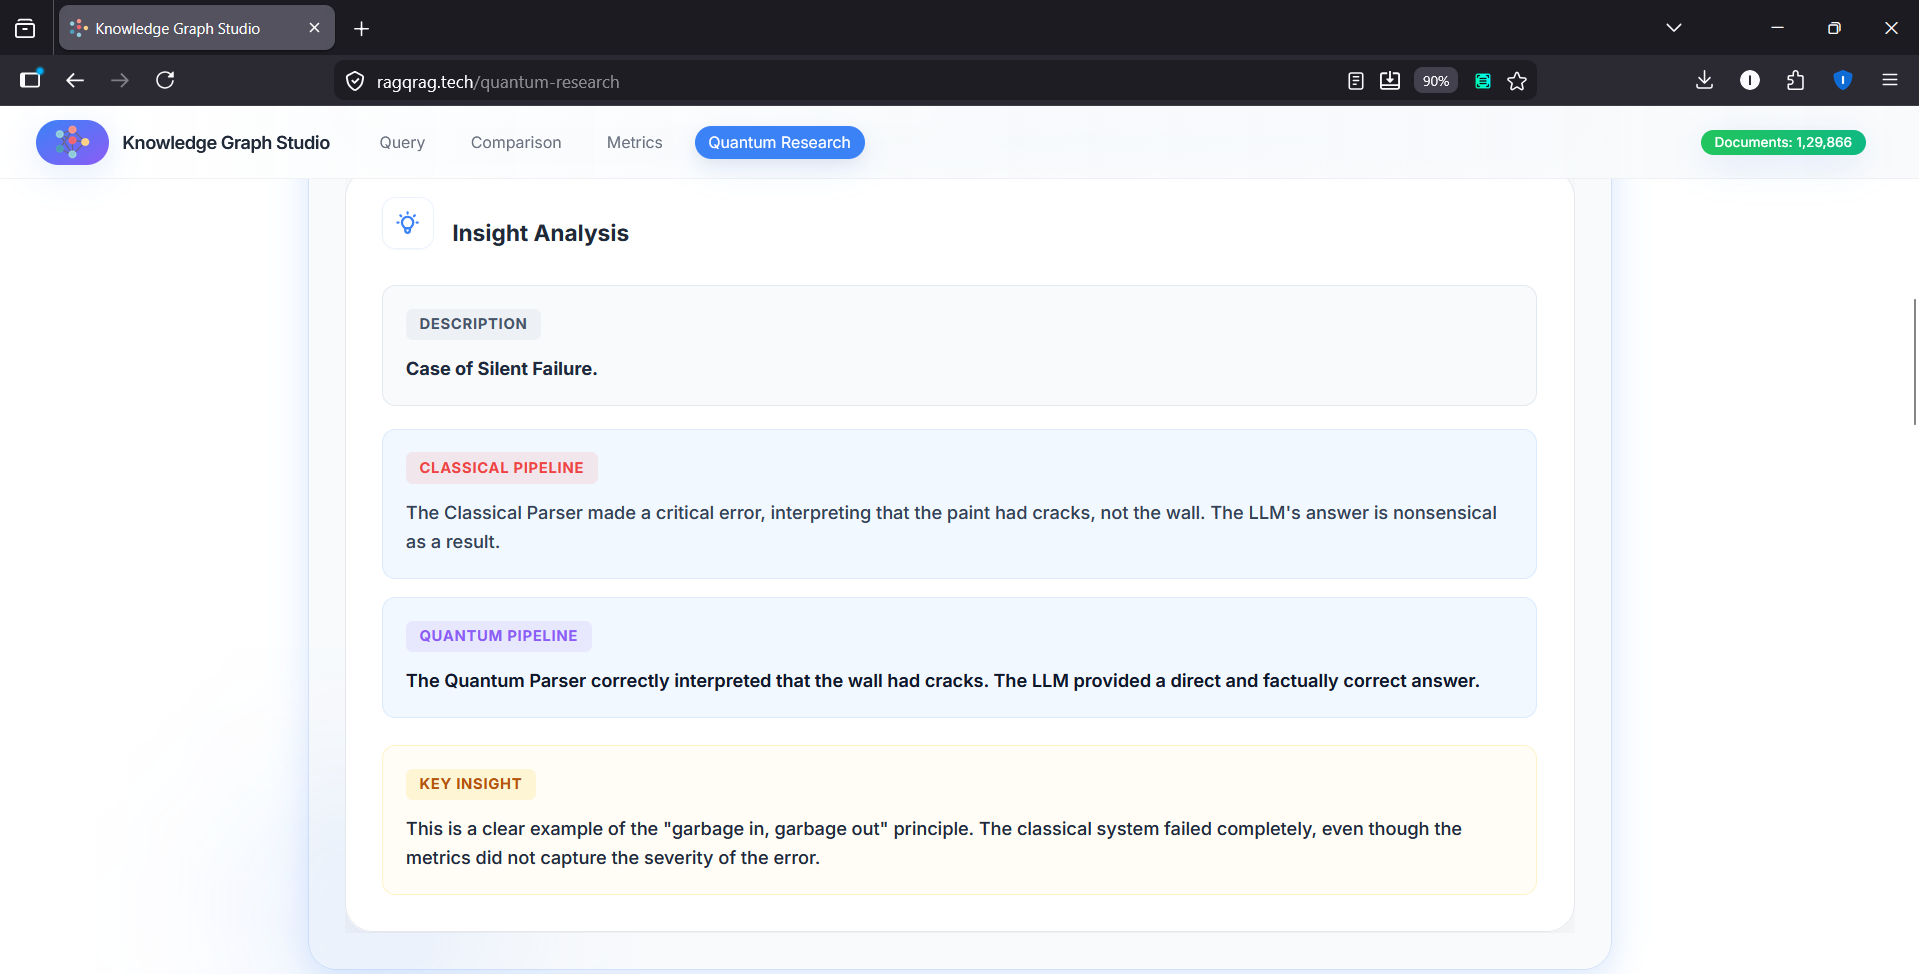
\includegraphics[width=0.7\textwidth]{assets/website/Quantum Research/insight analysis for the query.png}
	\caption{Website Section for Quantum Research}
	\label{fig:quantum}
\end{figure}

As shown in Figure~\ref{fig:advantage_vs_complexity_scatter} through a scatter diagram, a definite positive correlation exists. The advantage of quantum technology is not significant for straightforward semantic tasks (low complexity) because of the hardware noise that adversely affects its performance. Conversely, as syntactic complexity increases, like the presence of recursive clauses and deep prepositional phrases, classical algorithms struggle, while the quantum advantage becomes increasingly pronounced.

\begin{figure}[htbp]
	\centering
	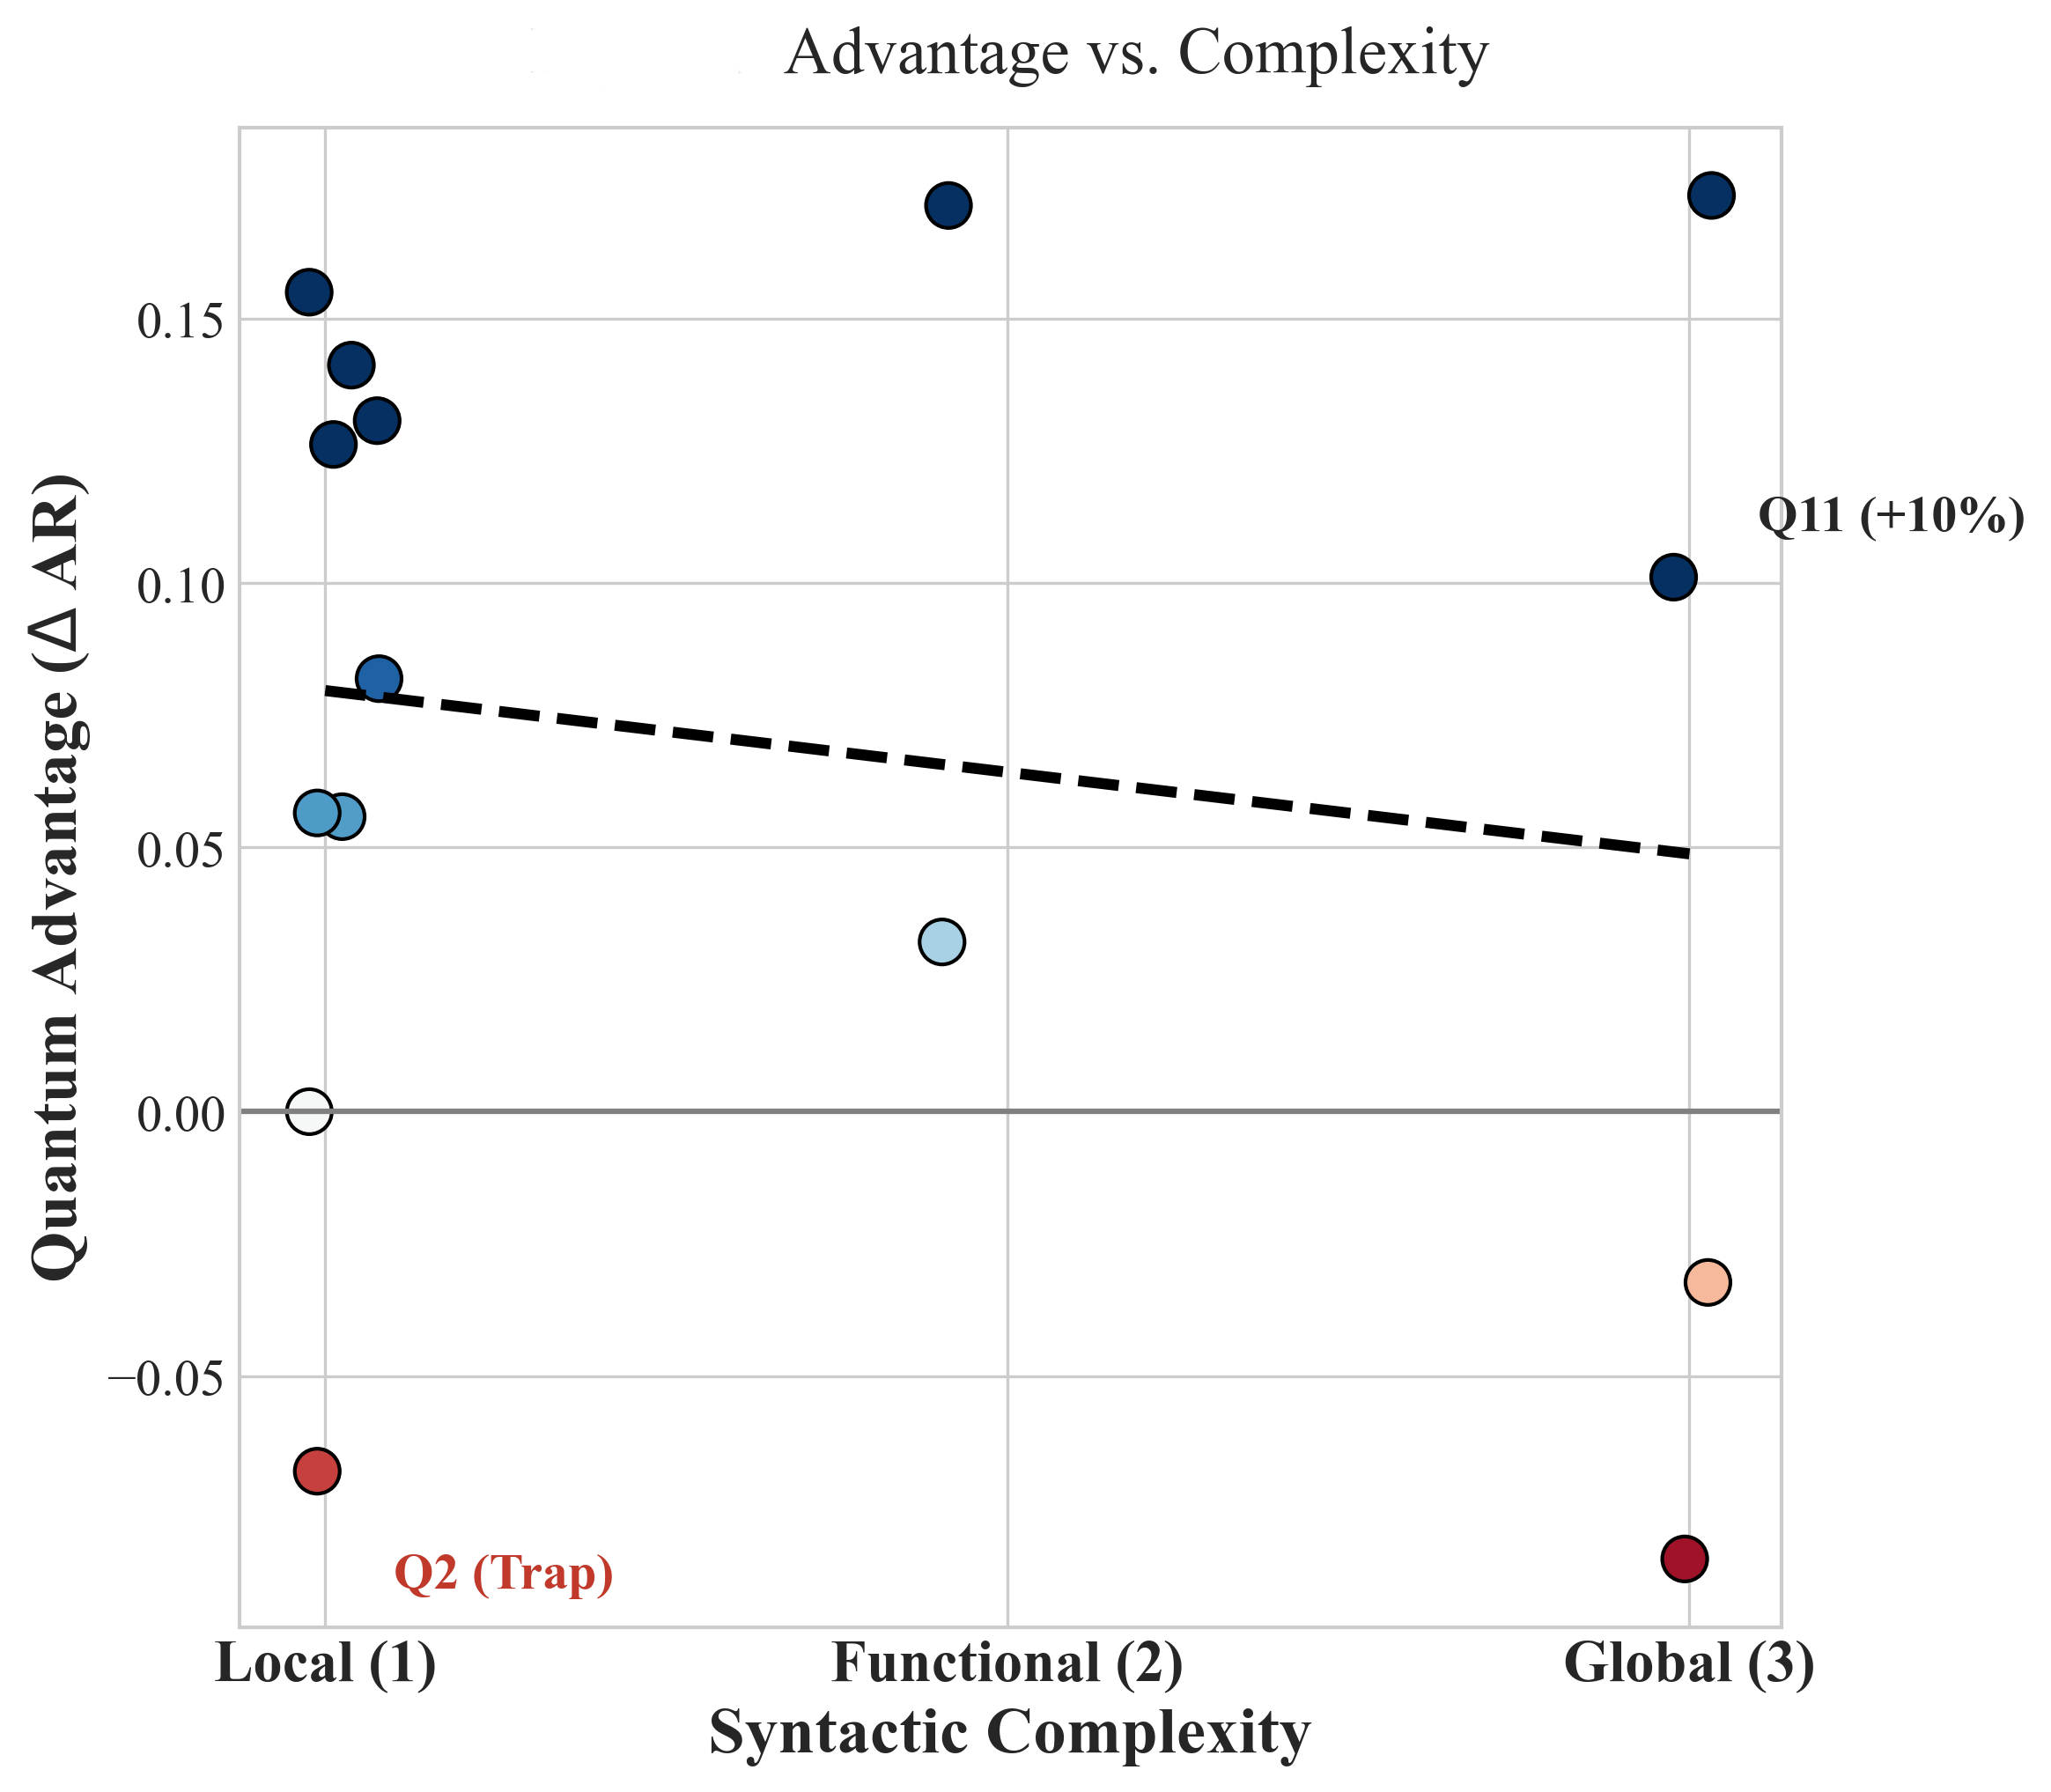
\includegraphics[width=0.7\textwidth]{assets/Journal/figure4.png}
	\caption{Scatter plot depicting the direct relationship between query syntactic complexity and the realized quantum advantage.}
	\label{fig:advantage_vs_complexity_scatter}
\end{figure}

\subsection{Edge Case Analysis \& Mobile View}

The user interface (UI) includes an edge case assessment environment. In the case of a user entering a query that is entirely irrelevant to the 130,000-document dataset, the retrieval components fail correctly. Figure~\ref{fig:edge_case} depicts an instance where the baseline Plain LLM model, which relies exclusively on parametric memory, generates a fluently articulated reply compared to the retrieval-enabled pipelines, emphasizing the rigidity of the architecture's domain containment property.

\begin{figure}[htbp]
	\centering
	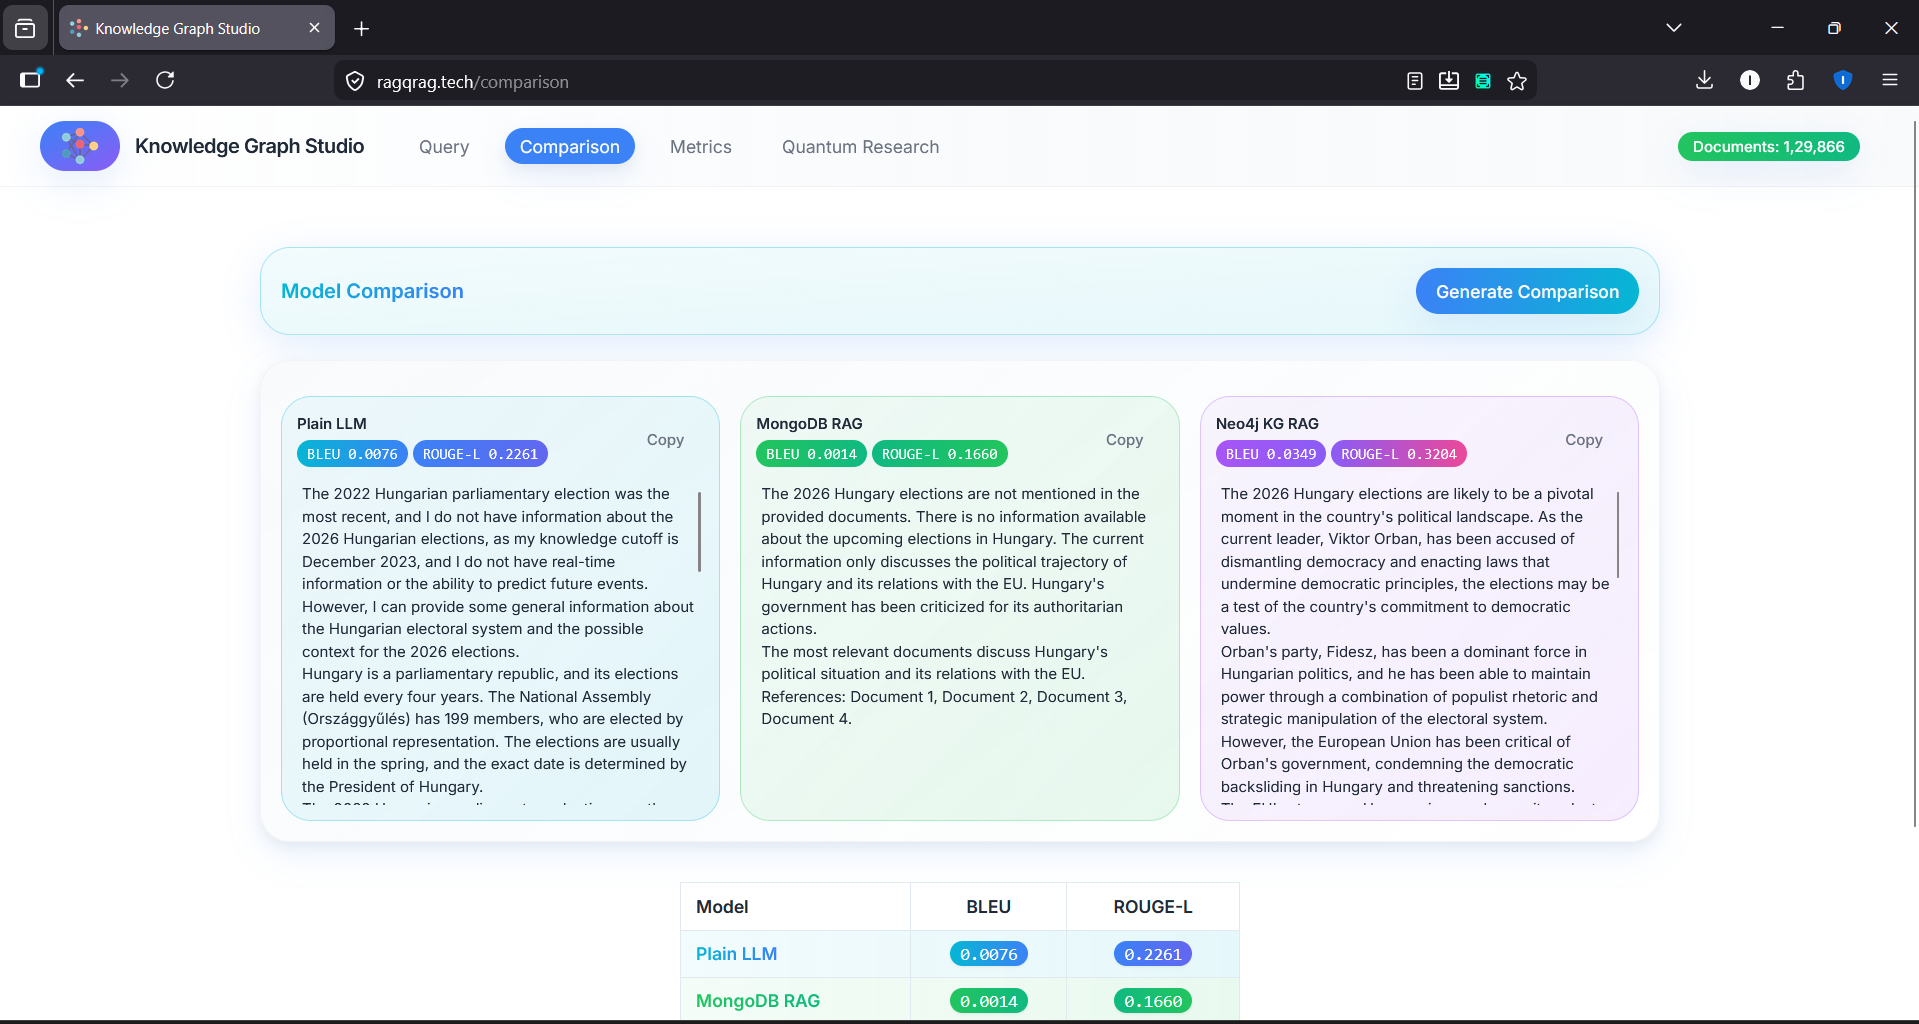
\includegraphics[width=0.8\textwidth]{assets/website/Unrelated query yields better plainLLM answer/model comparison.png}
	\caption{Edge case comparison interface demonstrating the baseline LLM outperforming the hybrid RAG system on out-of-domain queries.}
	\label{fig:edge_case}
\end{figure}

The website has also been modified to support mobile devices. Figure~\ref{fig:mobile_photos} show the seamless UI specially built for mobile devices.

\begin{figure}[htbp]
	\centering
	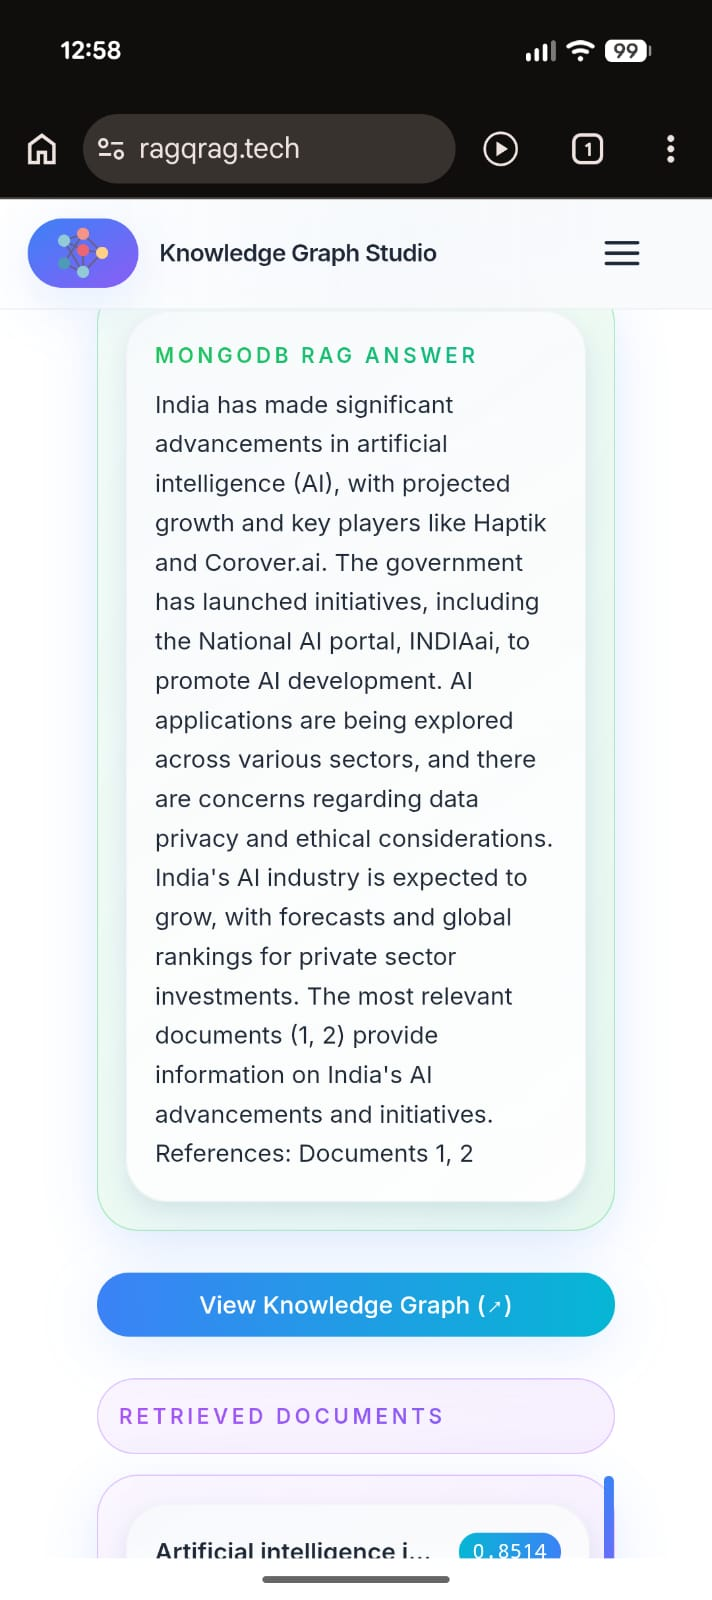
\includegraphics[width=0.3\textwidth]{assets/website/Mobile/mobile view query results.jpeg}
	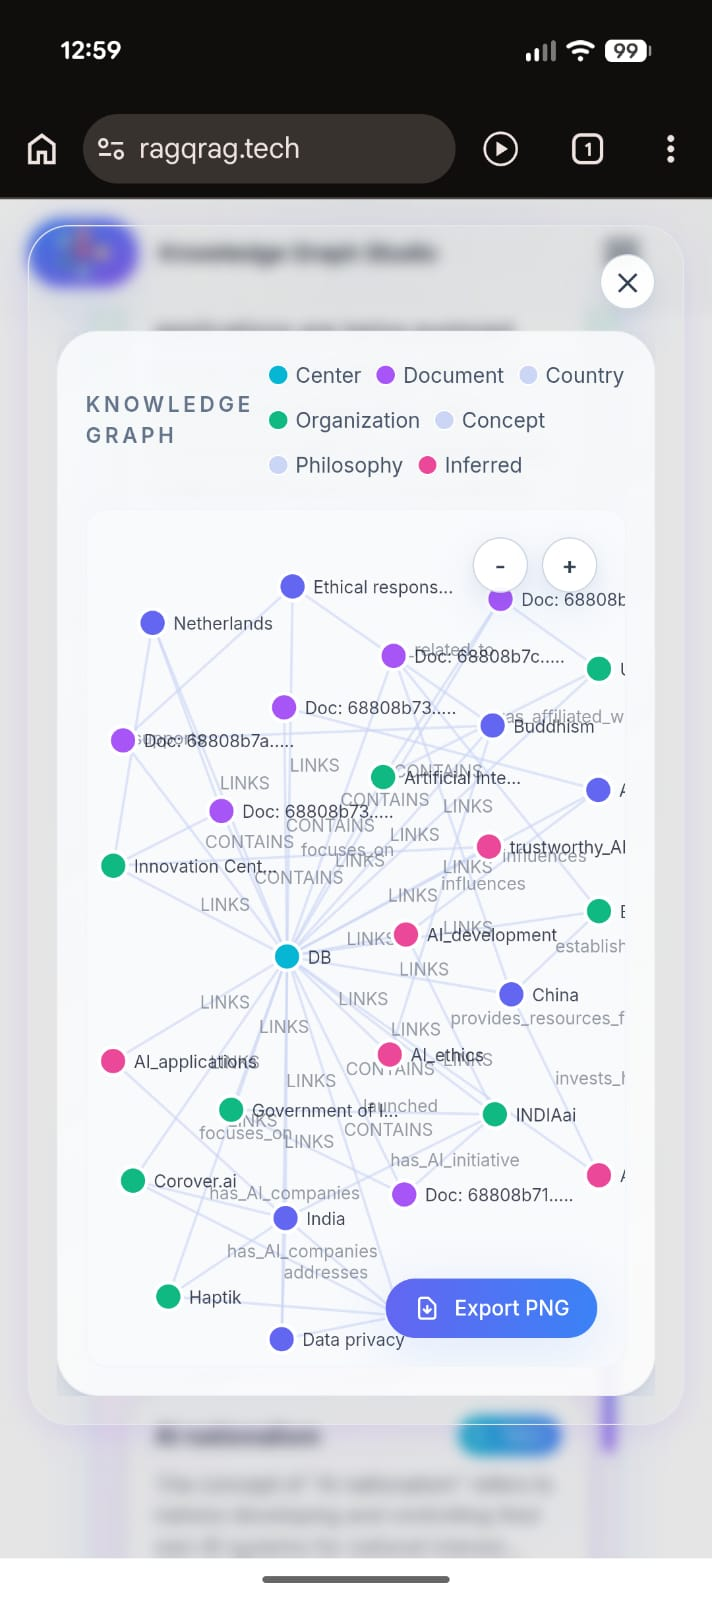
\includegraphics[width=0.3\textwidth]{assets/website/Mobile/mobile view graph pop up button .jpeg}
	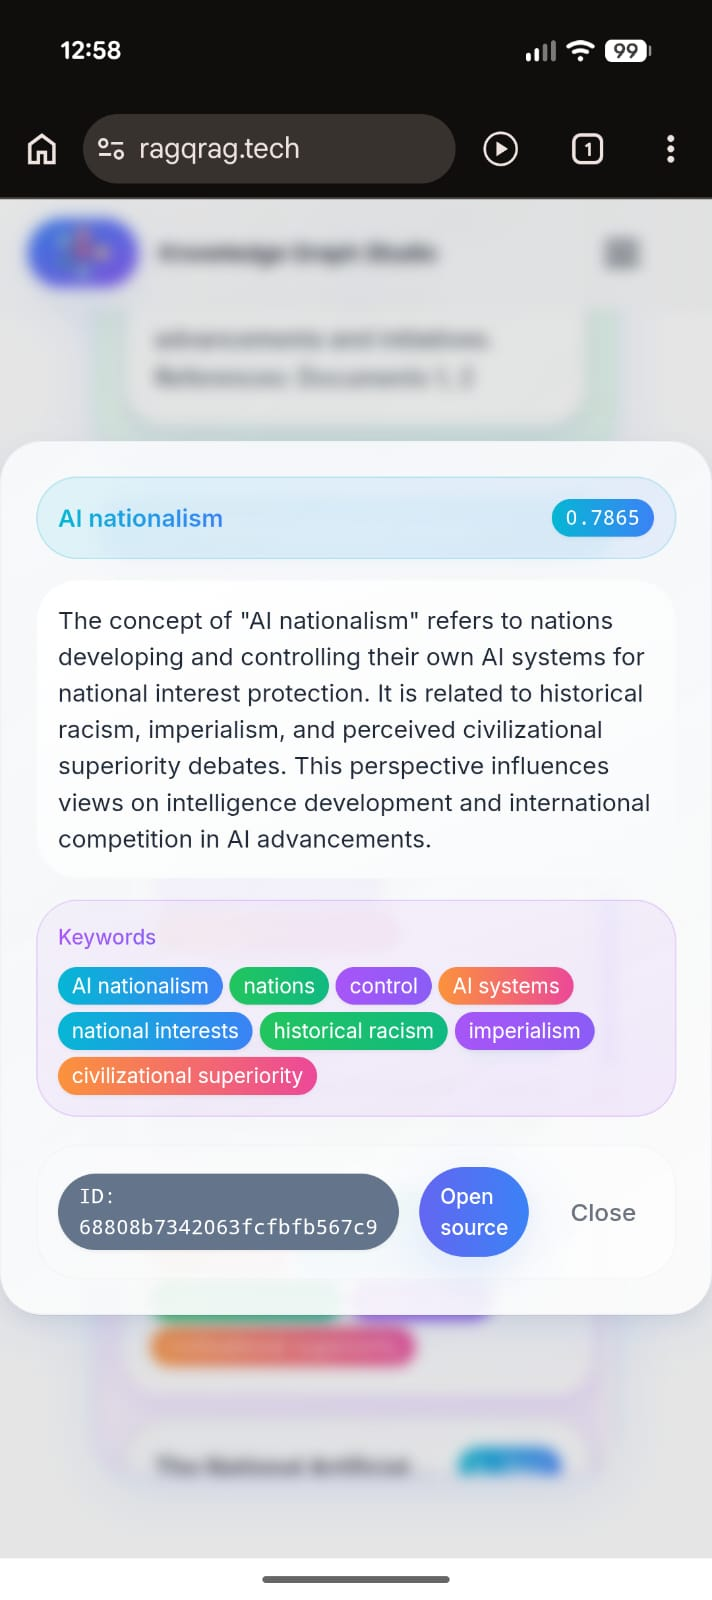
\includegraphics[width=0.3\textwidth]{assets/website/Mobile/mobile view clicked on a document.jpeg}
	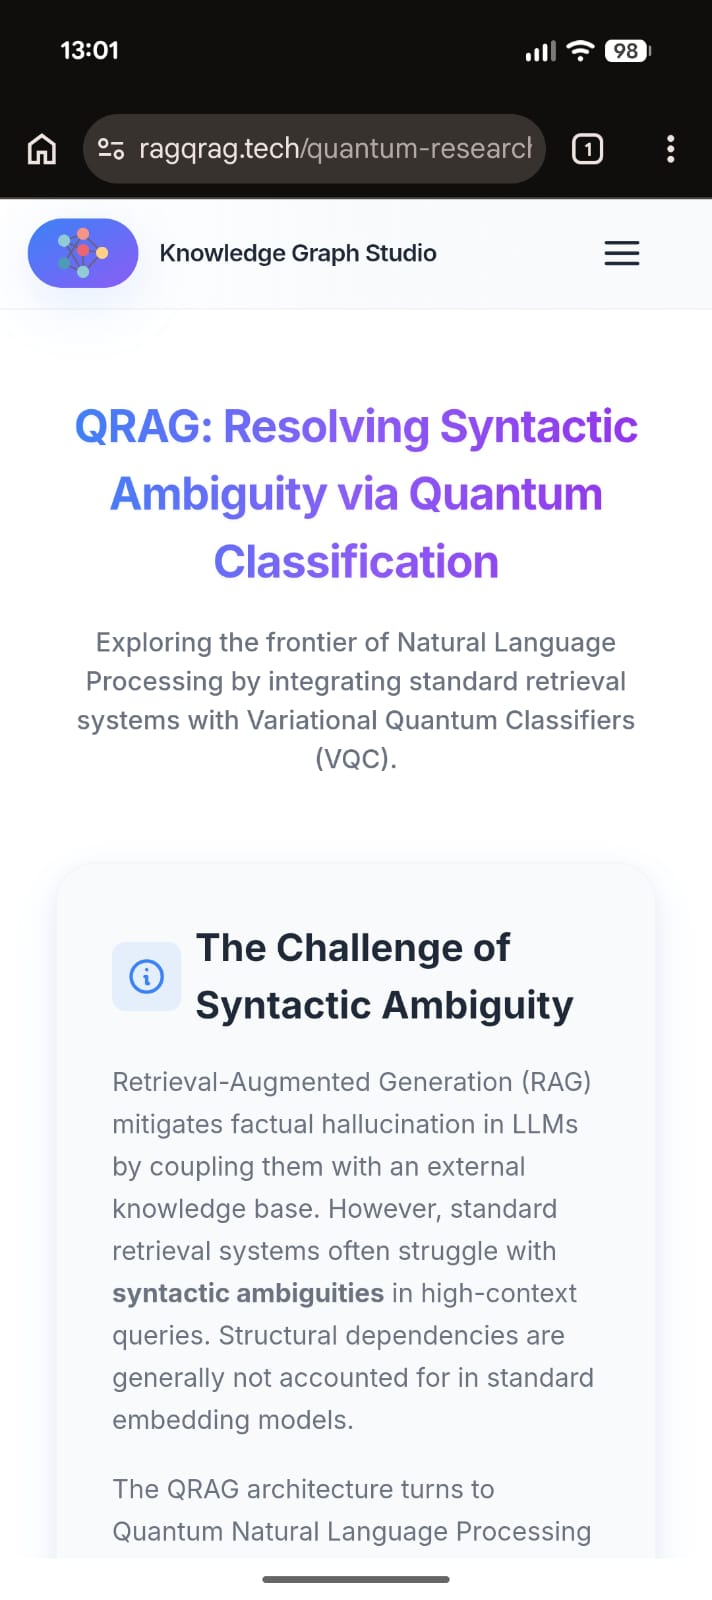
\includegraphics[width=0.3\textwidth]{assets/website/Mobile/mobile view quantum research homepage.jpeg}
	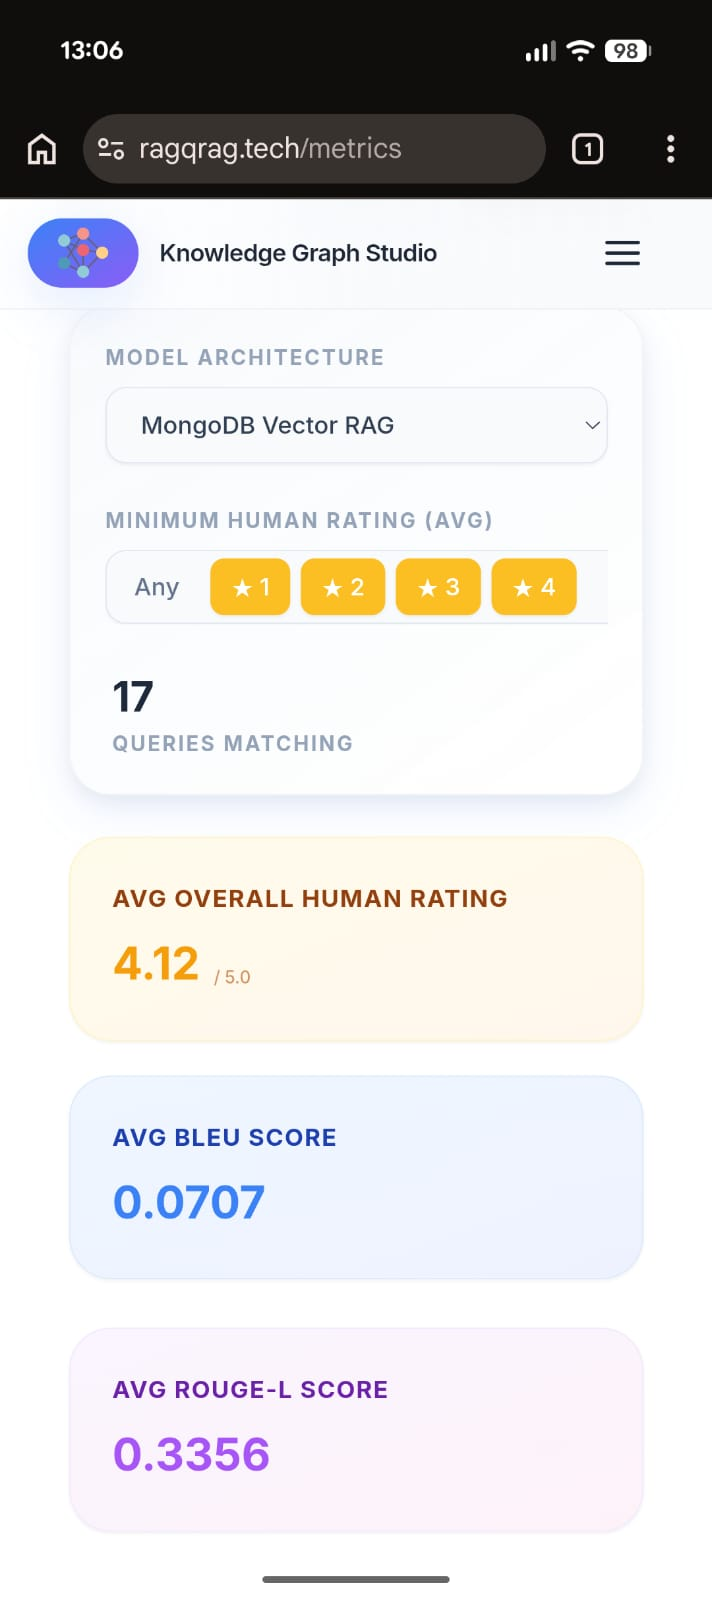
\includegraphics[width=0.3\textwidth]{assets/website/Mobile/mobile view metrics filter n view.jpeg}
	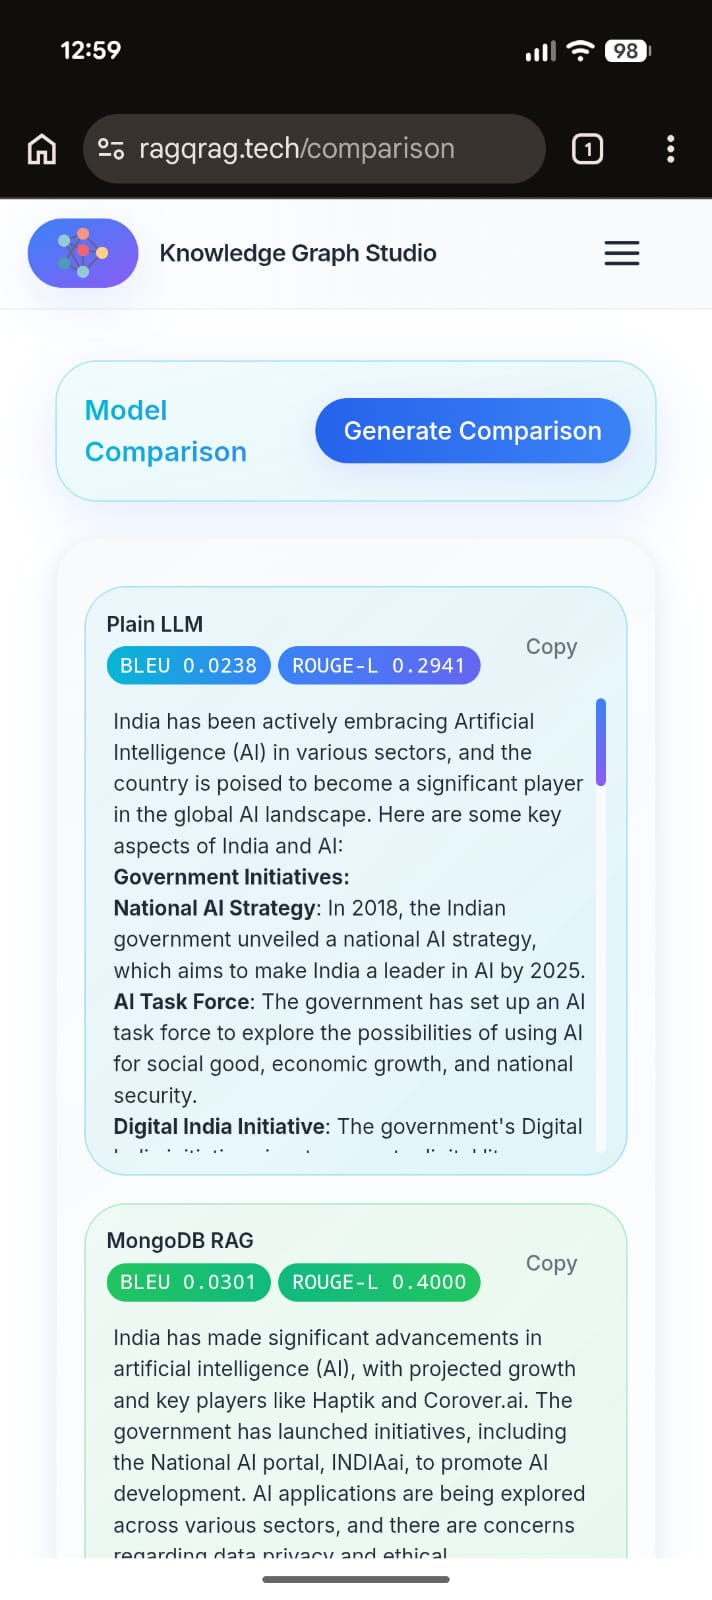
\includegraphics[width=0.3\textwidth]{assets/website/Mobile/mobile view comparison homepage.jpeg}
	\caption{Mobile View for the Website featuring special features like Graph Pop-Up window, etc.}
	\label{fig:mobile_photos}
\end{figure}

\section{Conclusion}

The empirical data affirm the hybrid architecture that comprises two entities. The classical approach, notably vector-based RAG equipped with constructive hallucinations, acts as a reliable primary machine and offers unbeatable performance in semantic searches conducted linearly. However, there exists a clear utility limitation within such classical engines. After recognizing the Linearity Trap and routing structurally uncertain queries through the novel QRAG engine, the system manages to avoid classical local attachment biases effectively. Consequently, it establishes a perfect harmony between classical heuristics, which are used to perform high-speed semantic searches, and quantum entanglements, which help interpret deep meanings when classical approaches cannot do so. The developed website successfully converts these research discoveries into a functional user interface tool.